\documentclass[aspectratio=169]{beamer}
\usepackage[utf8]{inputenc}
\usepackage{newunicodechar}
\newunicodechar{₹}{\textit{(INR)}}
\usepackage{tikz}
\usepackage{hyperref}
\usepackage{tabularx}
\usepackage{booktabs}  
\newcolumntype{Y}{>{\centering\arraybackslash}X}
\usetikzlibrary{shapes,arrows.meta,positioning}
\usepackage{supertabular}
\usepackage{array}
\usepackage{graphicx}
\usepackage{ragged2e}
\usepackage[backend=biber,style=ieee]{biblatex}
\addbibresource{references.bib}
\usetheme{Madrid} 
\setbeamertemplate{caption}[numbered]
\setbeamerfont{caption}{size=\footnotesize}

% Counter for figures
\setcounter{figure}{0}

\author[Aditya S T (P24DS005)]{%
Presented By:
\textbf{Aditya Sham Thombare (P24DS005)}
Guided By:
\textbf{Dr. Chandra Prakash}
\large Sardar Vallabhbhai National Institute of Technology
\large Surat, Gujarat 395007

\includegraphics[width=0.18\textwidth]{d0.png}}

\setbeamertemplate{title page}{
    \begin{beamercolorbox}[wd=\linewidth,ht=1.0cm,center,shadow=true,rounded=true]{title}
        \usebeamerfont{title}\inserttitle
    \end{beamercolorbox}

    \begin{center}
        \large \textbf{M. Tech - II Data Science (2024-26)} \\[0.8em]
        Presented By: Aditya Sham Thombare (P24DS005) \\ 
        Guided By: Dr. Chandra Prakash 
    \end{center}

    \begin{center}
        
\includegraphics[width=0.15\textwidth]{d0.png}
    \end{center}

    \begin{center}
        Department of Computer Science and Engineering\\[0.8em]
        Sardar Vallabhbhai National Institute of Technology, Surat \\[0.8em]
        \textbf{Dec 08, 2025}
    \end{center}
}

% Title text
\title{3D Reconstruction for CBCT with Enhanced X-Ray Images}

\begin{document}

\begin{frame}
    \titlepage
\end{frame}

% Outline Slide
\begin{frame}{Outline}
    \tableofcontents
\end{frame}

% Section 1
\section{Introduction}

\begin{frame}{Introduction: Importance of Oral Health}

\begin{columns}[T]
% -------- Left column --------
\column{0.45\textwidth}
\begin{itemize}
    \item Healthy teeth and gums are essential for proper chewing, clear speech,
    and overall quality of life.
    
    \item Oral health is closely linked to systemic health, with poor dental hygiene
    associated with conditions such as cardiovascular disease, diabetes,
    and infections.

    \item Dental imaging plays a critical role in early detection of cavities,
    bone loss, impacted teeth, and structural abnormalities.
\end{itemize}



% -------- Right column --------
\column{0.55\textwidth}
\begin{figure} 
    \centering 
    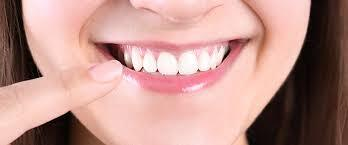
\includegraphics[width=0.85\textwidth]{Healthy.jpg}
    \caption{Healthy Teeth} 
    \label{fig:HealthyTeethy} 
\end{figure}

\end{columns}

\end{frame}

\begin{frame}{Introduction: Terminologies in the Domain}

\small
\begin{columns}[T,onlytextwidth]

    % ------------ LEFT SIDE (TEXT) ------------
    \begin{column}{0.50\textwidth}
        \begin{itemize}
            \item \textbf{Dentistry} — Branch of medicine concerned with diagnosis, prevention, and treatment of diseases of the teeth, gums, and oral cavity.

            \item \textbf{Periodontology} — Dental specialty focused on prevention, diagnosis, and treatment of diseases affecting supporting structures of teeth.

            \item \textbf{DRR (Digitally Reconstructed Radiograph)} — A synthetic 2D X-ray generated by projecting a 3D volume, commonly used for imaging simulation and data alignment.

            \item \textbf{Dentin} — Mineralized tissue beneath enamel forming the bulk of the tooth, sensitive to pain and decay.

            \item \textbf{Caries} — Tooth decay caused by bacterial acid leading to demineralization of enamel and dentin.

            \item \textbf{Periodontitis} — Advanced gum disease causing inflammation, bone loss, and potential tooth loss.

            \item \textbf{Prophylaxis} — Preventive dental procedures aimed at maintaining oral health and removing plaque and calculus.
        \end{itemize}
    \end{column}

    % ------------ RIGHT SIDE (IMAGE) ------------
    \begin{column}{0.50\textwidth}
        \begin{figure}
            \centering
            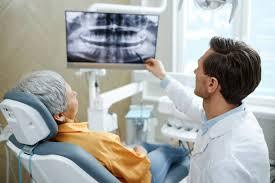
\includegraphics[width=0.85\textwidth]{download (2).jpg}
            \caption{Dental checkup}
            \label{fig:Checking}
        \end{figure}
    \end{column}

\end{columns}

\end{frame}

\begin{frame}{Introduction: Dental Anatomy \& Teeth Structure}

\small
\begin{columns}[T,onlytextwidth]

    % ------------ LEFT SIDE (TEXT) ------------
    \begin{column}{0.50\textwidth}
        \begin{itemize}
            \item \textbf{Dentition anatomy} — shows arrangement of incisors, canines,premolars and molars.
            \item \textbf{Tooth internal layers} — enamel (hard outer layer), dentin (supportive layer), and pulp
            \item \textbf{Supporting structures} — gums protect roots; periodontal ligament anchors teeth.
            \item \textbf{Jaw bone anatomy} — alveolar bone holds tooth sockets and maintains stability.
        \end{itemize}
    \end{column}

    % ------------ RIGHT SIDE (IMAGES) ------------
    \begin{column}{0.50\textwidth}
        \begin{figure}
            \centering
            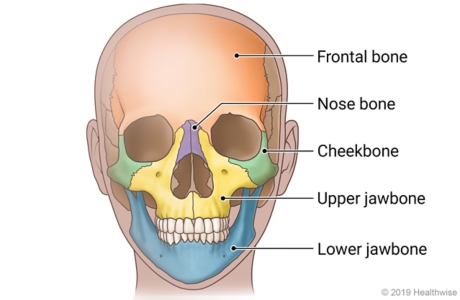
\includegraphics[width=0.55\textwidth]{jawbone.jpg}
            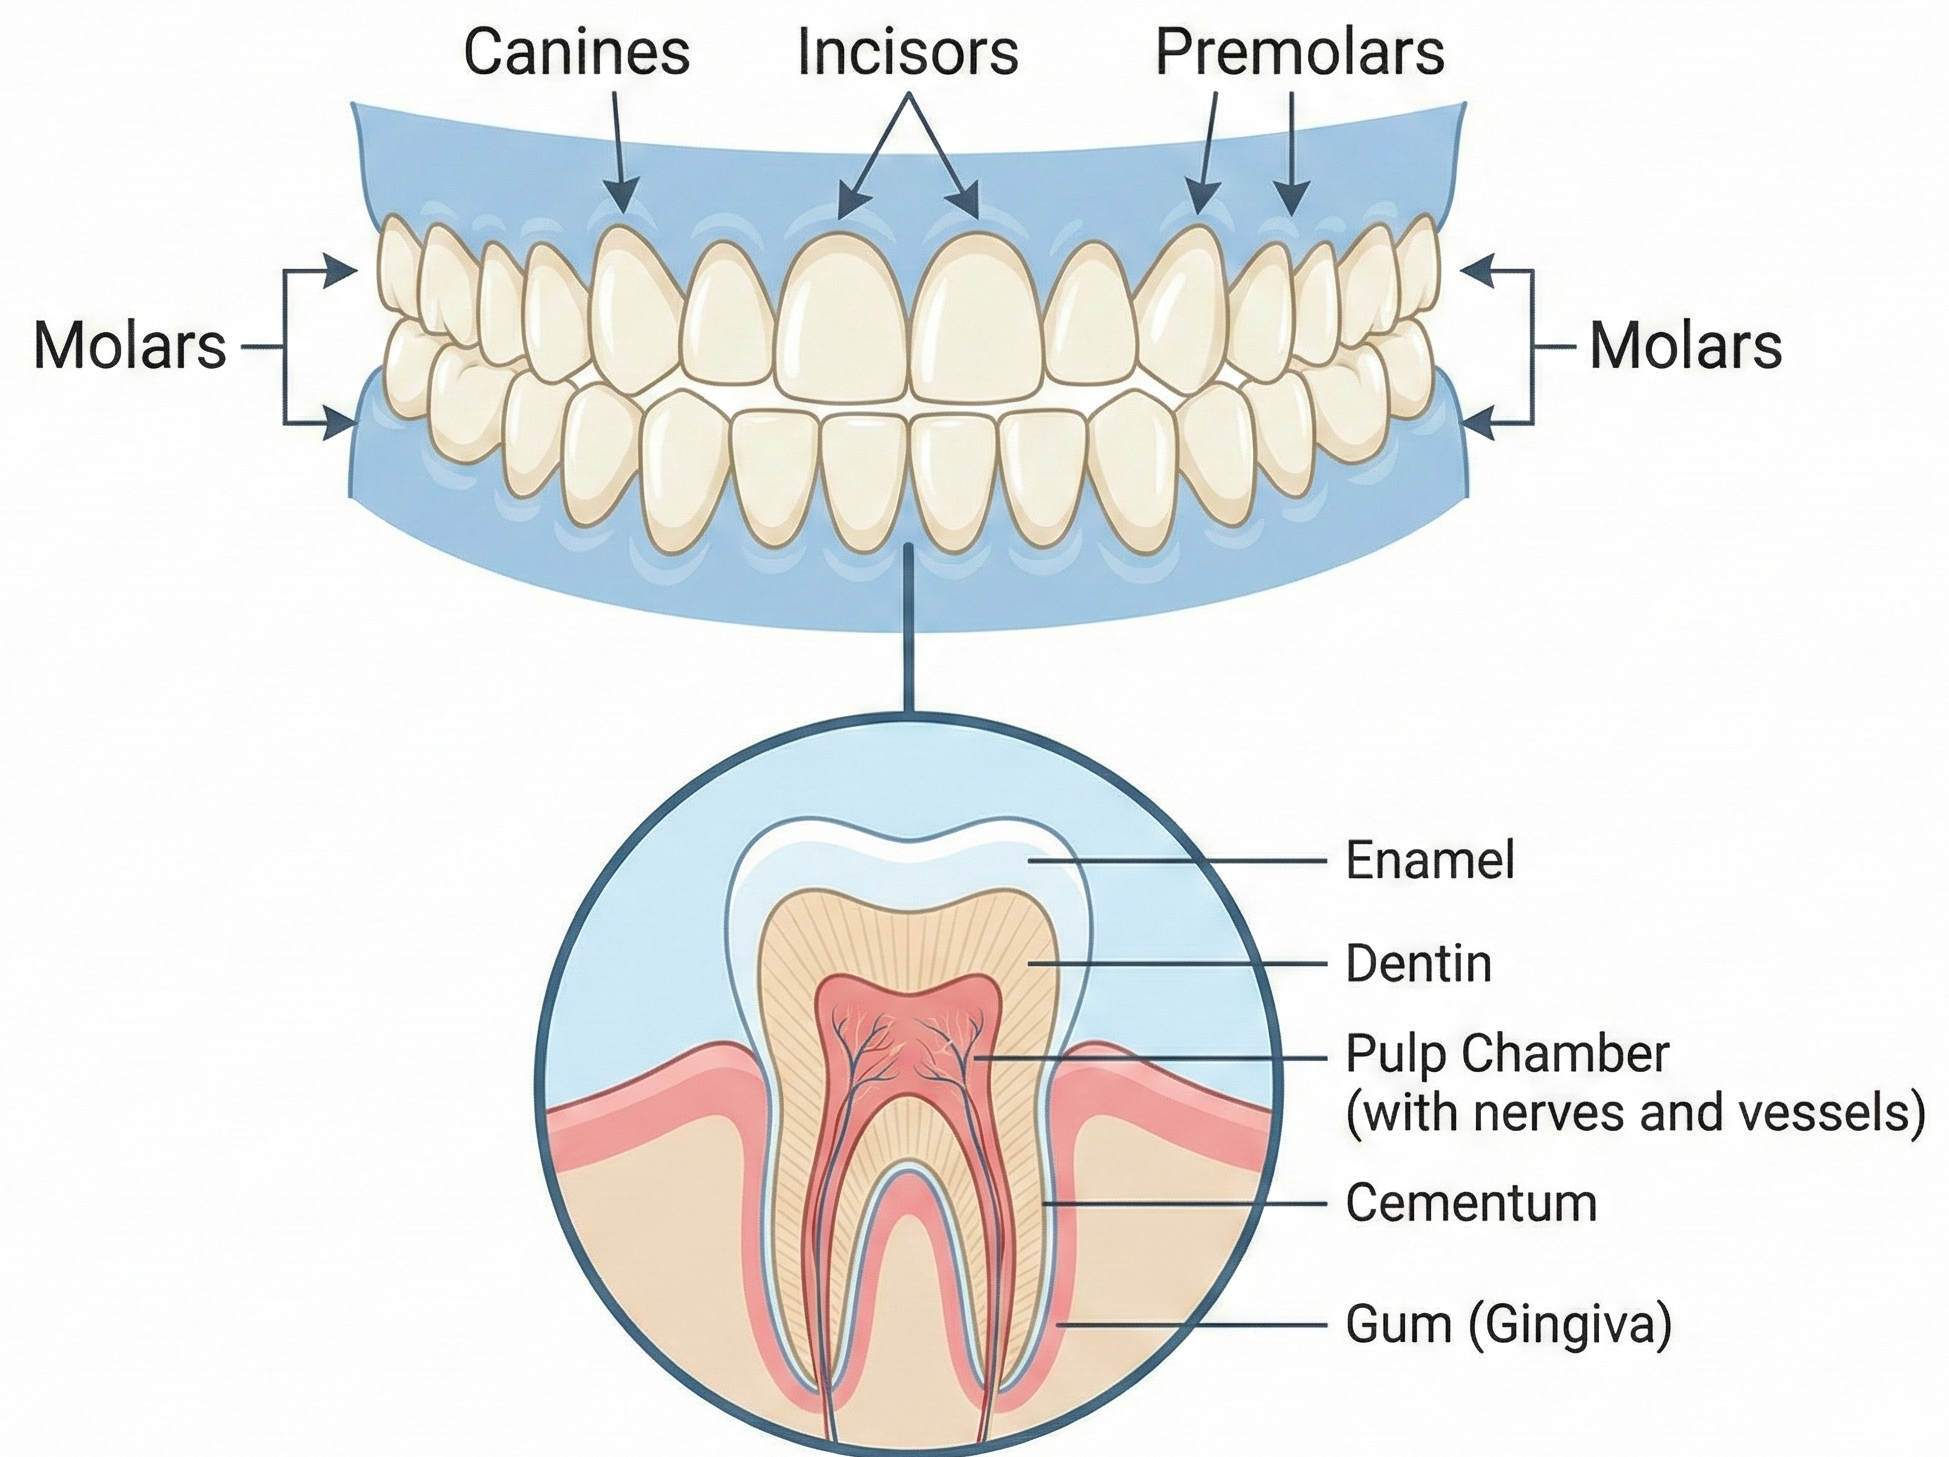
\includegraphics[width=0.55\textwidth]{tooth_Anatomy2.jpg.png}
            \caption{Dentition anatomy}
            \label{fig:dentition-anatomy}
        \end{figure}
    \end{column}

\end{columns}

\end{frame}

\begin{frame}{Major Dental Problems}

\begin{columns}[T,onlytextwidth]

    % ---------------- LEFT COLUMN (TEXT) ----------------
    \begin{column}{0.45\textwidth}
        \small
        \textbf{Common Dental Problems}
        \begin{itemize}
            \item \textbf{Dental caries (tooth decay):} Breakdown of enamel due to plaque, sugar, and poor oral hygiene.
            \item \textbf{Gingivitis and periodontitis:} Gum inflammation leading to bleeding, recession, and bone loss if untreated.\cite{anusree2023deep}
            \item \textbf{Tooth sensitivity:} Pain or discomfort triggered by hot, cold, sweet, or acidic foods caused by exposed dentin.\cite{ramesh2024machine}
            \item \textbf{Malocclusion (misaligned teeth):} Crowding, spacing, or bite problems affecting chewing and aesthetics.\cite{ma2024px2tooth}
        \end{itemize}
    \end{column}

    % ---------------- RIGHT COLUMN (IMAGES) ----------------
    \begin{column}{0.55\textwidth}
        \centering
        \begin{figure}
            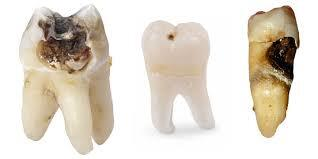
\includegraphics[width=0.75\textwidth]{images2.jpg}\\[4pt]
            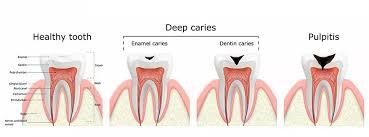
\includegraphics[width=0.85\textwidth]{images.jpg}
            \caption{Common dental issues illustrated}
            \label{fig:dental-issues}
        \end{figure}
    \end{column}

\end{columns}

\end{frame}

\begin{frame}{Diagnostic Methods for Dental Problems}

\small
\begin{columns}[T,onlytextwidth]

    % ---------------- LEFT COLUMN (TEXT) ----------------
    \begin{column}{0.55\textwidth}
        \textbf{Common Diagnostic Approaches in Dentistry}
        \begin{itemize}
            \item \textbf{Clinical Examination} — Visual and tactile inspection using mirrors and probes to detect caries, gum inflammation, bleeding, and bite irregularities.

            \item \textbf{Dental X-rays} — Includes bitewing, periapical, and panoramic radiographs for detecting hidden caries, bone loss, root infections, and impacted teeth.

            \item \textbf{Cone Beam CT (CBCT)} — Provides high-resolution 3D imaging for implant planning, complex extractions, root canal evaluation, and jaw pathology analysis.

            \item \textbf{Advanced Diagnostic Tools} — Intraoral cameras, laser-based caries detection, pulp vitality tests, and transillumination for early and precise diagnosis.
        \end{itemize}
    \end{column}

    % ---------------- RIGHT COLUMN (VERTICAL IMAGE STACK) ----------------
    \begin{column}{0.45\textwidth}
        \centering
        \begin{figure}
            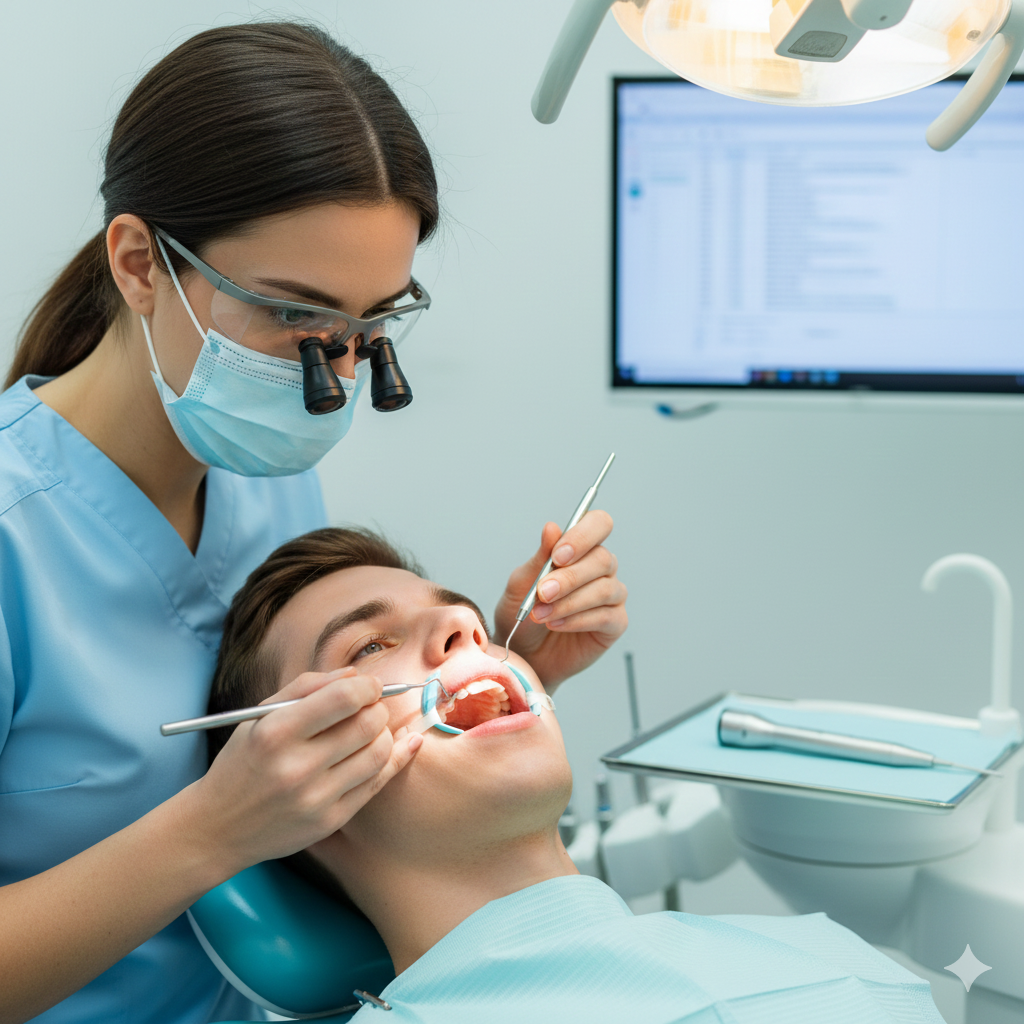
\includegraphics[width=0.34\textwidth]{normal.png}\\[4pt]
            \includegraphics[width=0.34\textwidth]{Xraydoctor.png}\\[4pt]
            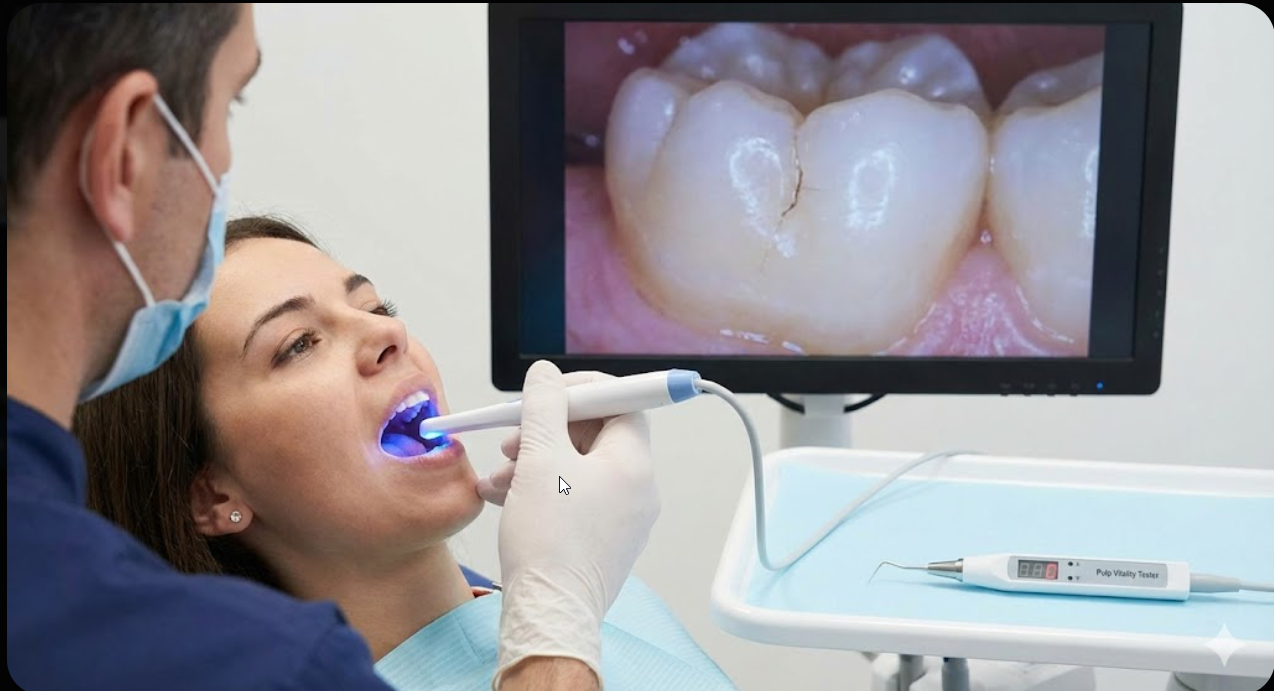
\includegraphics[width=0.34\textwidth]{InCamera.png}
            \caption{Dental diagnostic methods}
            \label{fig:dental-diagnostics}
        \end{figure}
    \end{column}

\end{columns}

\end{frame}


\begin{frame}{Digitally Reconstructed Radiograph}

\small
\centering
\begin{table}
\renewcommand{\arraystretch}{1.3}
\begin{tabular}{|p{3cm}|p{5cm}|p{4cm}|}
\hline
\textbf{Type of X-ray} & \textbf{Purpose / What it Shows} & \textbf{Key Use} \\
\hline
Bitewing (BWX) & Shows the crowns of upper and lower posterior teeth in a single image. 
& Detecting cavities between teeth and evaluating bone levels. \\
\hline
Periapical (PA) & Shows the entire tooth from crown to root apex along with surrounding bone. 
& Diagnosing root abscesses, bone loss, and pulp-related issues. \\
\hline
Panoramic (Pan) & Provides a wide view of the entire mouth, jaws, teeth, and TMJ. 
& Assessing impacted wisdom teeth, cysts, tumors, and overall development. \\
\hline
Cone Beam CT (CBCT) & Provides detailed three-dimensional cross-sectional images. 
& Implant planning, complex extractions, and advanced endodontic treatment. \\
\hline
\end{tabular}
\end{table}

\end{frame}

\begin{frame}{DRR on Imaging Data }
    \begin{figure}
        \centering
        \includegraphics[width=0.85\textwidth]{infoarc.jpg}
        \caption{Different Modules on Imaging Data}
        \label{fig:drr-imaging}
    \end{figure}
\end{frame}
    

\begin{frame}{What are X-Ray Images?}
    \begin{itemize}
        \item A single, flattened image created by passing X-rays through the body. 
        It shows overlapping structures, losing depth information. \\[2pt]

        \textit{Example: A panoramic X-ray Teeth Labels}
    \end{itemize}

    \begin{figure}
        \centering
        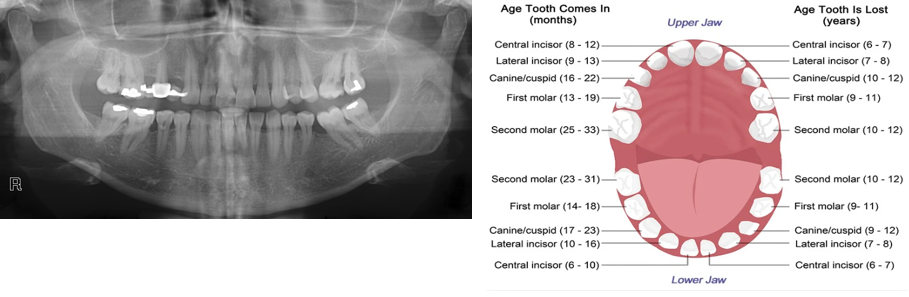
\includegraphics[width=0.85\textwidth]{XrayTeeth.png}
        \caption{Panoramic dental X-ray and Teeth Labels}
        \label{fig:panoramic-xray}
    \end{figure}

    \footnotesize Source: \url{https://youtu.be/YfhaFfozTvQ?si=DTDJzZ1OkDyeCsuM}
\end{frame}

\begin{frame}{What are CBCT Images?}

\begin{itemize}
    \item \textbf{CBCT (Cone-Beam Computed Tomography - 3D):} 
    A 3D imaging technique where an X-ray source rotates around the patient,
    capturing hundreds of 2D projections that are reconstructed into a 
    detailed 3D volume.

    \item These reconstructions allow clinicians to view the anatomy in 
    multiple planes: axial, coronal, sagittal, and as a 3D model.
\end{itemize}

\vspace{0.2cm}

\begin{figure}
    \centering
    \begin{tabular}{cccc}
        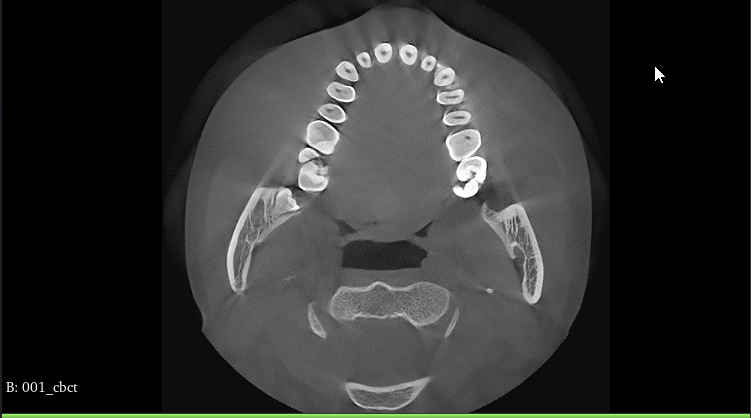
\includegraphics[width=0.23\textwidth]{v1.png} &
        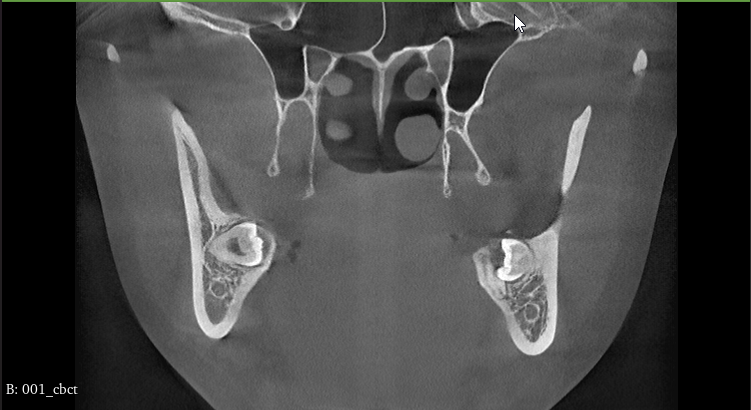
\includegraphics[width=0.23\textwidth]{v2.png} &
        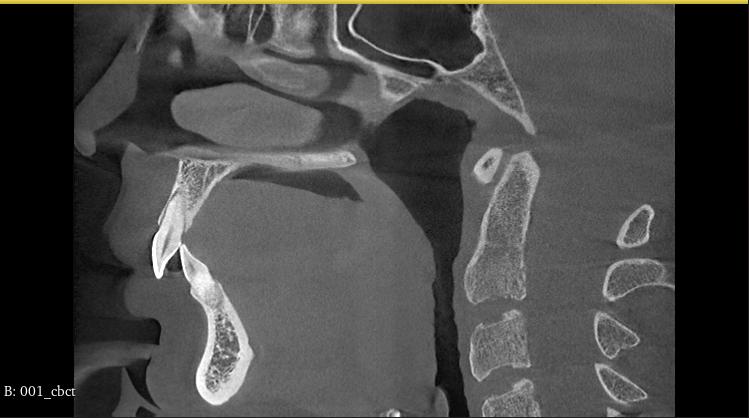
\includegraphics[width=0.23\textwidth]{v3.png} &
        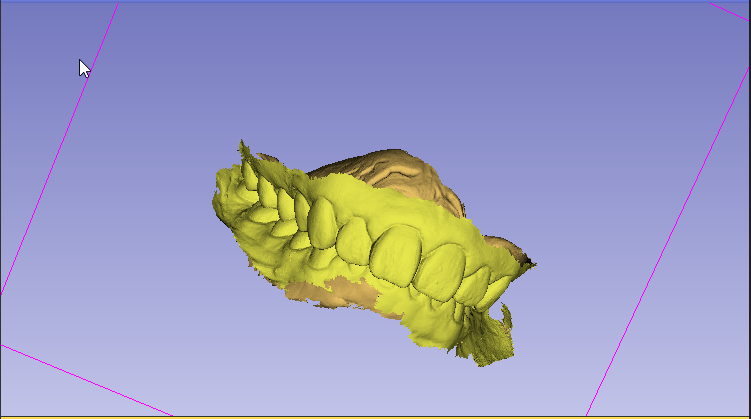
\includegraphics[width=0.23\textwidth]{v4.png} \\
        \footnotesize Axial View &
        \footnotesize Coronal View &
        \footnotesize Sagittal View &
        \footnotesize 3D Mesh
    \end{tabular}
    \caption{CBCT multi-planar views and 3D reconstruction}
    \label{fig:cbct-views}
\end{figure}

\footnotesize Source: \url{https://youtu.be/eLlYEEU-wUA?si=29Arb8i0eL9mPk_n}

\end{frame}

\section{Literature Survey}

\begin{frame}[fragile]{Literature Survey}
\centering
\scriptsize
\resizebox{\textwidth}{!}{%
\begin{tabular}{ p{5.0cm} p{3.4cm} p{3.5cm} p{5.0cm} }
\toprule
\textbf{Paper Title \& Year} & \textbf{Techniques} & \textbf{Evaluation Metric (Best)} & \textbf{Comments / Drawbacks} \\
\midrule

NeRF: Representing Scenes as Neural Radiance Fields (2020) &
Fully-connected deep MLP network for volumetric rendering and view-synthesis &
PSNR / SSIM / LPIPS:  
42.65 / 0.991 / 0.047 (best) &
Very slow training (1–2 days/scene), slow inference (~30s/frame), requires dense multi-view images and accurate camera poses. \\
\addlinespace[4pt]

X2Teeth (2021) – 3D Teeth Reconstruction from a Single PX &
Multi-subnetwork CNN: SegNet + ReconNet &
IoU / DA / DF:  
X2Teeth: \textbf{0.682 / 0.702 / 0.747} &
Depends on synthetic PX from CBCT; limited real clinical data; low accuracy for incisors/wisdom teeth. \\
\addlinespace[4pt]

Attention U-Net for Flattened CBCT Reconstruction (2023) &
Attention U-Net reconstructs flattened 3D CBCT from PX &
\textbf{Ablation Study (2023)}  
PSNR: 16.68–16.80  
SSIM: 61–73\%  
Dice: 61–73\% &
Uses flattened-CBCT (not true 3D volume); performance depends heavily on synthetic data quality. \\
\addlinespace[4pt]

3DPX Review (2023) — 2D→3D X-ray Reconstruction Review &
Comprehensive survey of 20+ 2D→3D methods &
Best reported:  
ResNet50 Acc 98.84\%, F1 97.65\%  
ConvNeXtNano Acc 96.84\%, F1 98.14\% &
General survey; limited dental-specific focus. \\
\addlinespace[4pt]


Neural Radiance Fields in Medical Imaging: A Survey (2024) &
Survey of NeRF-based medical reconstruction (MedNeRF, UMedNeRF, NAF, SNAF) &
Qualitative survey (no fixed metric) &
High dependency on paired data; difficulty reconstructing fine anatomical detail; boundary ambiguity; computationally heavy; limited modality generalization. \\
\addlinespace[4pt]

NeBLa: Neural Beer–Lambert Model (2024) &
CycleGAN → SimPX; NeRF-like 3D reconstruction guided by Beer–Lambert physics &
\textbf{Quantitative (2024)}  
PSNR: 19.89 → 21.68  
SSIM: 79.21\% → 82.62\%  
Dice: 65.22\% → 74.77\% &
Two-stage pipeline; assumes heuristic X-ray trajectory; requires unpaired PX for style translation; computationally heavy. \\
\bottomrule
\end{tabular}%
}
\label{tab:literature-survey-1}
\end{frame}


\begin{frame}[fragile]{Literature Survey (continued)}
\centering
\scriptsize
\resizebox{\textwidth}{!}{%
\begin{tabular}{ p{5.0cm} p{3.4cm} p{3.5cm} p{5.0cm} }
\toprule
\textbf{Paper Title \& Year} & \textbf{Techniques} & \textbf{Evaluation Metric (Best)} & \textbf{Comments / Drawbacks} \\
\midrule

NeBLa: Neural Beer–Lambert Model (2024) &
CycleGAN → SimPX; NeRF-like 3D reconstruction guided by Beer–Lambert physics &
\textbf{Quantitative (2024)}  
PSNR: 19.89 → 21.68  
SSIM: 79.21\% → 82.62\%  
Dice: 65.22\% → 74.77\%  
LPIPS: 0.30 → 0.24 &
Two-stage pipeline; assumes heuristic X-ray trajectory; requires unpaired PX for style translation; computationally heavy. \\
\addlinespace[4pt]

PX2Tooth (2024) – 3D Point Cloud from PX &
Two-stage:  
PXSegNet (2D segmentation) + TGNet (3D point cloud via PFM) &
\textbf{Teeth-level IoU (FDI numbers)}  
Baseline Avg: 0.60–0.69  
PX2Tooth: \textbf{0.72–0.91 (best)} &
Reconstructs teeth only (not jawbone); point clouds need meshing; dataset/code not public. \\
\addlinespace[4pt]

3DPX (2024) – Progressive 2D→3D Reconstruction &
Hybrid MLP–CNN U-Net with progressive guidance &
\textbf{Quantitative (2024)}  
PSNR: 15.84  
DSC: 63.72  
SSIM: \textbf{74.09} (best) &
Complex architecture; computationally heavy; trained on synthetic PX from CBCT (limited real-world generalization). \\
\addlinespace[4pt]

Oral-3Dv2 (2025) – 3D Volume from PX &
Neural X-ray Field (NeXF) – implicit representation from single PX &
Accuracy: \textbf{88.33\%} &
Slow implicit querying; depends on precise X-ray path simulation; code not public. \\
\bottomrule
\end{tabular}%
}
\label{tab:literature-survey-2}
\end{frame}

\begin{frame}{History for Xrays and CBCT}

\begin{figure}[htbp]
\centering
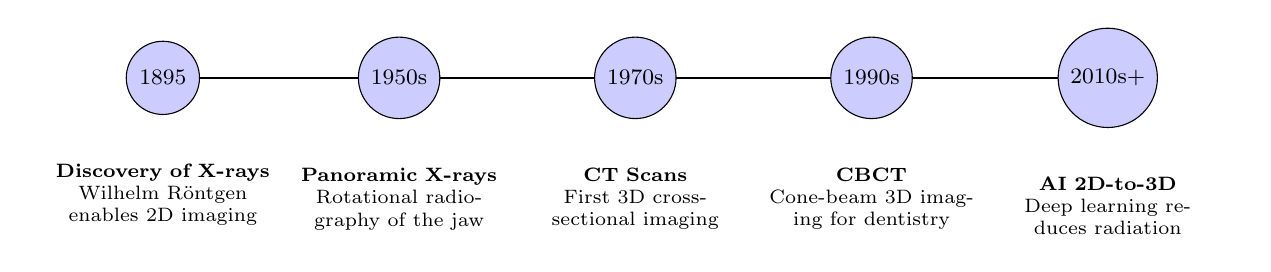
\begin{tikzpicture}[
    timeline/.style={
        circle, draw, fill=blue!20,
        minimum size=8mm, font=\footnotesize
    },
    label style/.style={
        text width=3.2cm,
        align=center,
        font=\scriptsize
    }
]

% Horizontal line
\draw[thick] (0,0) -- (12,0);

% Timeline nodes
\node[timeline] (x1895) at (0,0) {1895};
\node[timeline] (x1950) at (3,0) {1950s};
\node[timeline] (x1970) at (6,0) {1970s};
\node[timeline] (x1990) at (9,0) {1990s};
\node[timeline] (x2010) at (12,0) {2010s+};

% Labels below each node
\node[label style, below=0.5cm of x1895] {
    \textbf{Discovery of X-rays}\\
    Wilhelm Röntgen enables 2D imaging
};

\node[label style, below=0.5cm of x1950] {
    \textbf{Panoramic X-rays}\\
    Rotational radiography of the jaw
};

\node[label style, below=0.5cm of x1970] {
    \textbf{CT Scans}\\
    First 3D cross-sectional imaging
};

\node[label style, below=0.5cm of x1990] {
    \textbf{CBCT}\\
    Cone-beam 3D imaging for dentistry
};

\node[label style, below=0.5cm of x2010] {
    \textbf{AI 2D-to-3D}\\
    Deep learning reduces radiation
};

\end{tikzpicture}
\caption{Historical timeline of dental imaging technologies}
\label{fig:imaging-timeline}
\end{figure}

\end{frame}


\begin{frame}{Comparison of Dental Imaging: 2-D X-rays vs CBCT}

\small
\begin{table}[ht]
\centering
\begin{tabular}{|p{3cm}|p{2.7cm}|p{3.2cm}|p{4.2cm}|}
\hline
\textbf{Imaging Modality} & 
\textbf{Typical Effective Dose} & 
\textbf{Equivalent to Natural Radiation} &
\textbf{Advantages / Limitations} \\
\hline

Intraoral dental X-ray (single) &
1.5–8.2 µSv &
Less than 1 day of background radiation &
Low dose, simple; limited to 2D and may miss hidden canals or fractures \\ 
\hline

Panoramic 2-D X-ray &
4–30 µSv (typically ~20–25 µSv) &
~1–3 days of background radiation &
Broader view than intraoral; still 2D and may miss subtle 3D problems \\ 
\hline

Dental CBCT (small/medium FOV) &
20–200 µSv (modern low-dose often $\leq$50 µSv) &
A few days to ~2 weeks of background exposure &
3D imaging, high detail; detects hidden canals, fractures; dose depends strongly on FOV \\ 
\hline

Dental CBCT (large FOV / older systems) &
Up to 500–530 µSv &
Several weeks of background radiation &
High diagnostic value; higher radiation — must be justified, use smallest FOV \\ 
\hline

\end{tabular}
\caption{\href{https://www.endodonticexcellence.com/blog/why-modern-dental-x-rays-cbct-scans-are-safe/}{Comparison of radiation doses in dental imaging modalities}}
\label{tab:radiation-comparison}
\end{table}

\end{frame}

\begin{frame}{Dental X-Ray and CBCT Cost Summary}

\small
\begin{itemize}
    \item \textbf{Basic Dental X-ray (Periapical / RVG)} — ₹300–600 across India; Pune clinics typically charge ₹300–600.

    \item \textbf{Bitewing X-ray} — Costs range between ₹400–800; commonly ₹600 in Pune.

    \item \textbf{Panoramic X-ray (OPG)} — ₹800–1500 nationwide; Pune average around ₹1500.

    \item \textbf{CBCT (3D Imaging)} — ₹1500–5500 in India; Pune clinics commonly charge ₹2500–6000 depending on scan area.
\end{itemize}

\vspace{6pt}
\footnotesize
\textbf{Sources:} \\
\href{https://www.aodentistry.com/blog/dental-x-ray-cost/}{AO Dentistry – Dental X-ray Cost in India} \\
\href{https://www.aodentistry.com/dental-x-ray-in-pune/}{AO Dentistry – Dental X-ray Cost in Pune}

\end{frame}

\begin{frame}{AI/ML in Dental Images-Capabilities}
\begin{figure}
    \centering
    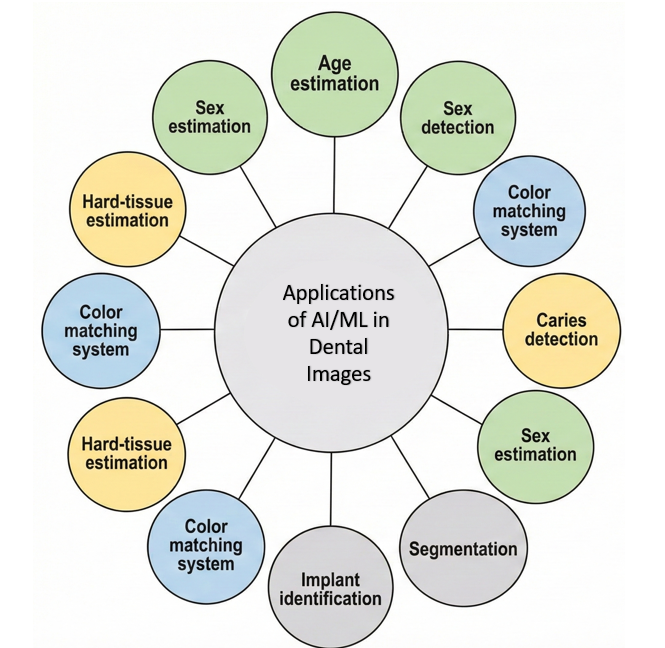
\includegraphics[width=0.44\textwidth]{AIML_in_Dental.png}
    \caption{AI/ML applications in dental imaging}
    \label{fig:ai-dental-applications}
\end{figure}
\end{frame}

\section{Research Gaps}

\begin{frame}{Research Gaps Identified}
\begin{itemize}
    \item \textbf{Scarcity of Paired Clinical Data}  
    The development of robust models is limited by the lack of large-scale, publicly available datasets containing paired 2D X-rays and 3D CBCT scans from the same patient.
    \item \textbf{Insufficient Clinical Utility and Robustness}  
    As reported by Mahesh et al. (2024), many evaluations focus on technical metrics instead of clinically relevant outcomes, making it difficult to validate robustness against pathologies, artifacts, and domain shifts.\cite{shin2025sparse}
    \item \textbf{Limited Reconstruction of Diagnostic Detail}  
    Current reconstruction methods fail to capture fine anatomical structures—such as root morphology and bone microstructure—required for diagnostic accuracy and clinical planning.\cite{ma2024px2tooth}
    \item \textbf{Assumption of Standardized X-ray Trajectory}  
    Many approaches rely on an idealized, fixed X-ray trajectory, which may not align with real-world variations across different clinical machines.\cite{song2021oral}
\end{itemize}
\end{frame}

\begin{frame}{Problem Statement and Objectives}

\begin{beamercolorbox}[rounded=true, shadow=true, sep=1em, wd=\textwidth]{block body}
\textbf{Problem Statement:}  
Low-quality 2D X-ray projections often contain noise, artifacts, and reduced contrast, which significantly degrade the accuracy and clarity of reconstructed 3D CBCT volumes.Enhanching 2D Xrays and Reconstruction of CBCT for reliable 3D views in in lower cost.
\end{beamercolorbox}

\vspace{0.4cm}

\textbf{Objectives:}
\begin{itemize}
    \item To reduce radiation exposure and improve accessibility for clinics lacking CBCT machines by enabling high-quality 3D reconstruction from enhanced 2D projections.
    
    \item To eliminate the reliance on large paired 2D--3D datasets and enhance the anatomical fidelity and diagnostic accuracy of reconstructed 3D CBCT volumes through advanced enhancement techniques.
\end{itemize}

\end{frame}

\begin{frame}{Dataset: CBCT and X-rays}
    \begin{itemize}
        \item We have 100 CBCT scans in NIfTI format, each paired with its corresponding 3D mesh in STL format.
        \item We possess 936 panoramic X-ray images.
        \item Of those, 156 X-rays are segmented.
    \end{itemize}

    \vspace{0.2cm}

    \begin{figure}
        \centering
        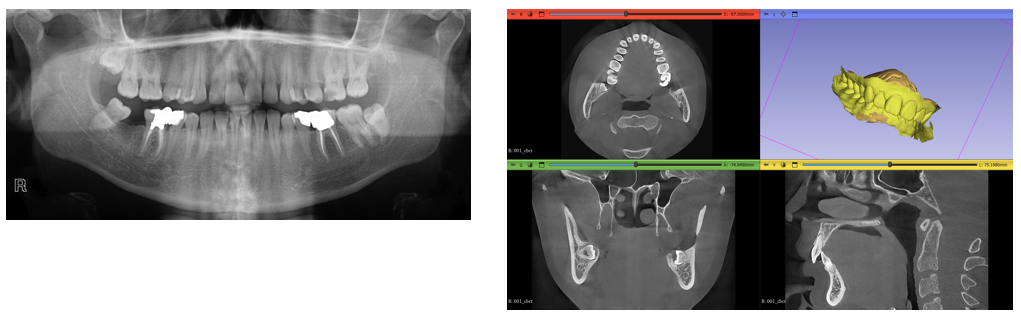
\includegraphics[width=0.9\textwidth]{d5.png}
        \caption{Dataset composition: CBCT scans and panoramic X-rays}
        \label{fig:dataset-composition}
    \end{figure}
\end{frame}

\section{Pilot Study}

\begin{frame}{Pilot Study: Initial Experiment}
\begin{figure}
\centering
    \includegraphics[width=1.04\textwidth]{NeblaArch.png}
    \caption{NeBLa Paper Approach}\cite{park2024nebla}
    \label{fig:pilot-study}
\end{figure}

\end{frame}

\begin{frame}{Pilot Study: Initial Experiment}
\begin{columns}[T]
    % Left column: Text
    \begin{column}{0.65\textwidth}
        \begin{itemize}
            \item \textbf{Slicing and Pre-processing of CBCT Images}
            \begin{itemize}
                \item 3D CBCT scan loaded from a NIfTI file, extracting the raw voxel data and affine matrix defining spatial orientation.
                \item Slice extraction performed from the axial view.\cite{park2024nebla}
            \end{itemize}

            \vspace{0.4cm}

            \item \textbf{Reconstructing the CBCT Using the Slices}
            \begin{itemize}
                \item Sequentially read saved 2D axial slices and stack them to reconstruct the 3D NumPy volume.
                \item A new NIfTI file is generated using the reconstructed volume along with original spatial metadata.
                \item Integrity of reconstruction is verified by comparing shape and voxel intensities to estimate data loss.\cite{park2024nebla}
            \end{itemize}
        \end{itemize}
    \end{column}

    % Right column: Image
    \begin{column}{0.35\textwidth}
        \begin{figure}
        \centering
        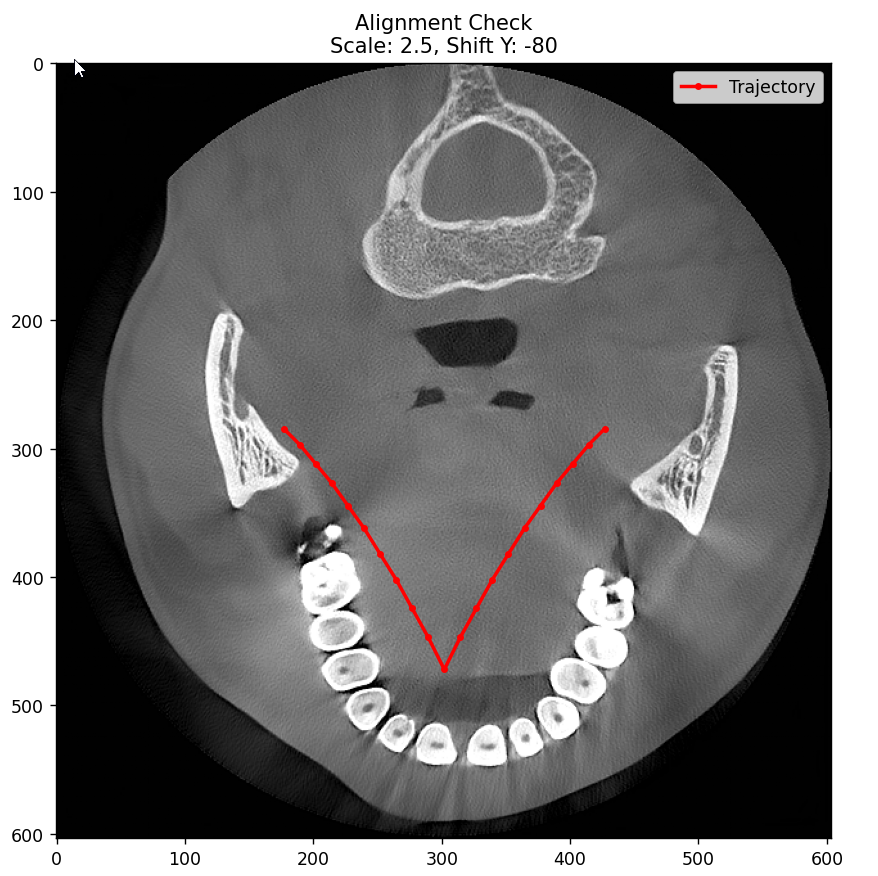
\includegraphics[width=\textwidth]{r0.png}
        \caption{Trajectory estimation}
        \label{fig:cbct-reconstruction-workflow}
        \end{figure}
    \end{column}
\end{columns}
\end{frame}


\section{Methodology}

% \begin{frame}{Methodology: CBCT to Panoramic DRR Architecture}
% \small
% \begin{itemize}
%     \item \textbf{Input}: CBCT volume loading (\texttt{.nii/.nii.gz}).
%     \item \textbf{Preprocessing}: Volume standardization and normalization.
%     \item \textbf{Arch Detection}: Dental arch extraction from bone voxels.
%     \item \textbf{DRR Engine}: Curved focal-trough ray tracing.
%     \item \textbf{PX Generation}: Panoramic X-ray synthesis.
%     \item \textbf{Augmentation}: Multi-view rotations and intensity jitter.
%     \item \textbf{Pairing}: Paired CBCT + synthetic PX dataset creation.
%     \item \textbf{Evaluation}: SSIM, PSNR, and MSE based quality checks.
%     \item \textbf{Output}: Final dataset and pipeline metrics.
% \end{itemize}
% \end{frame}

\begin{frame}{Methodology: CBCT Volume Processing Flow and Step Outputs}
\centering
\begin{figure}
    \centering
    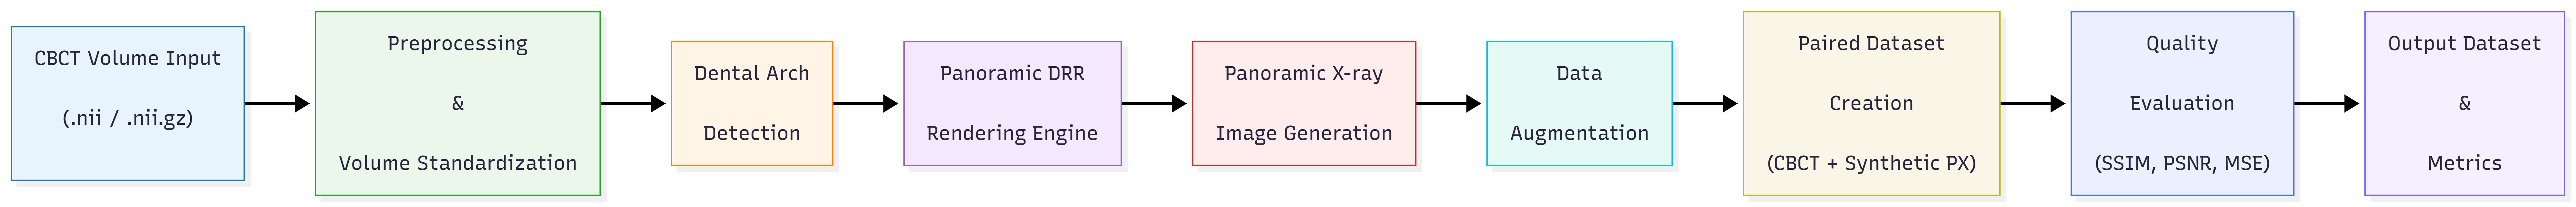
\includegraphics[width=0.98\textwidth]{CBCT Volume Processing.png}
    \vspace{-0.3cm}
    \scriptsize
    \begin{tabular}{ccccccccc}
        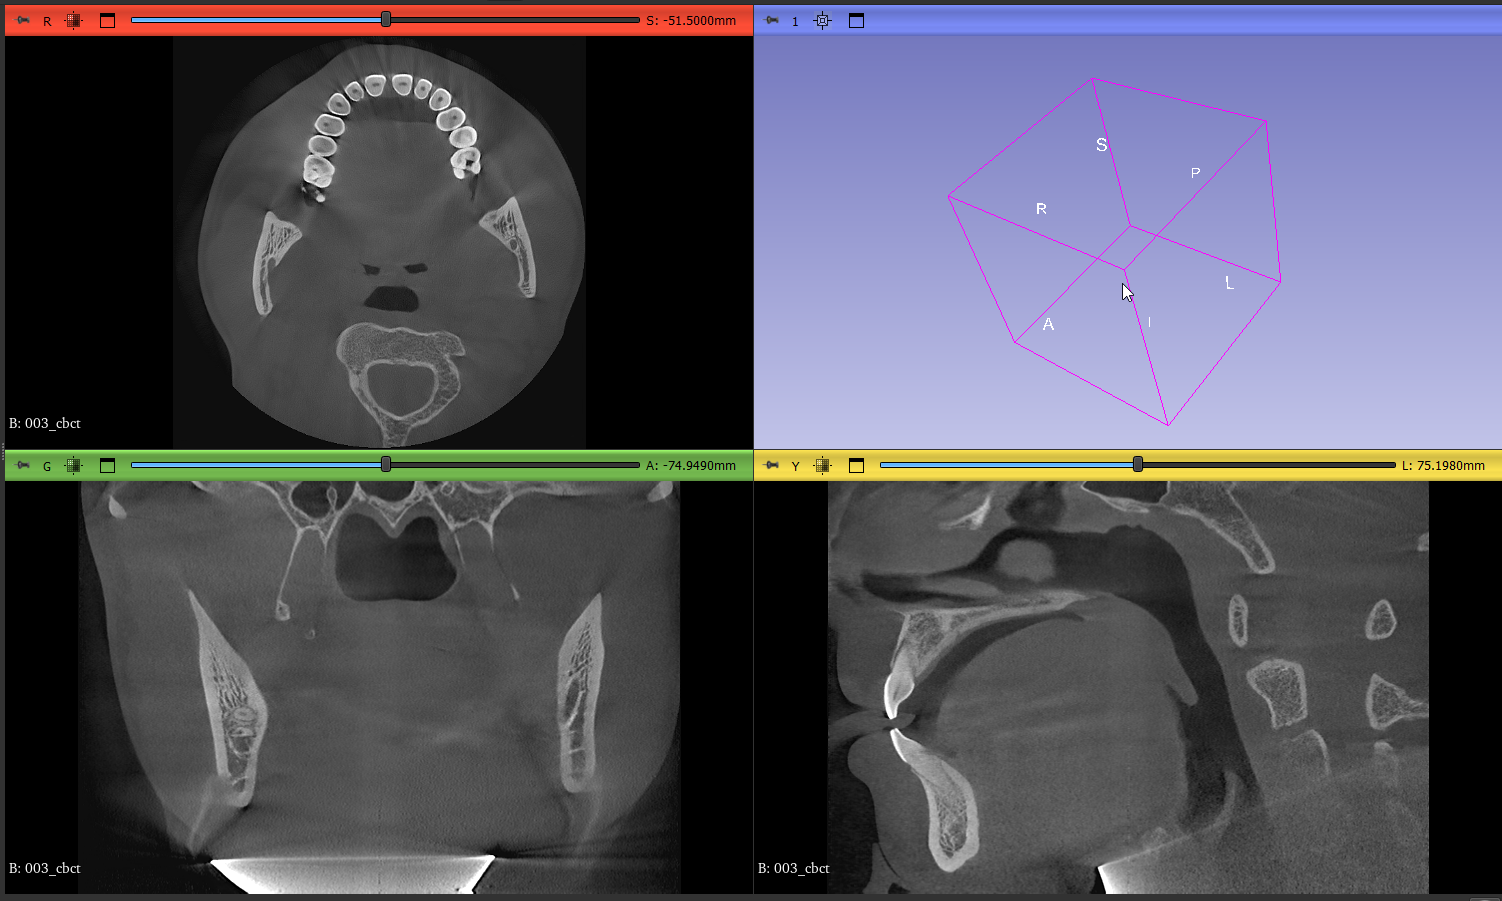
\includegraphics[width=0.10\textwidth]{cbct1.png} &
        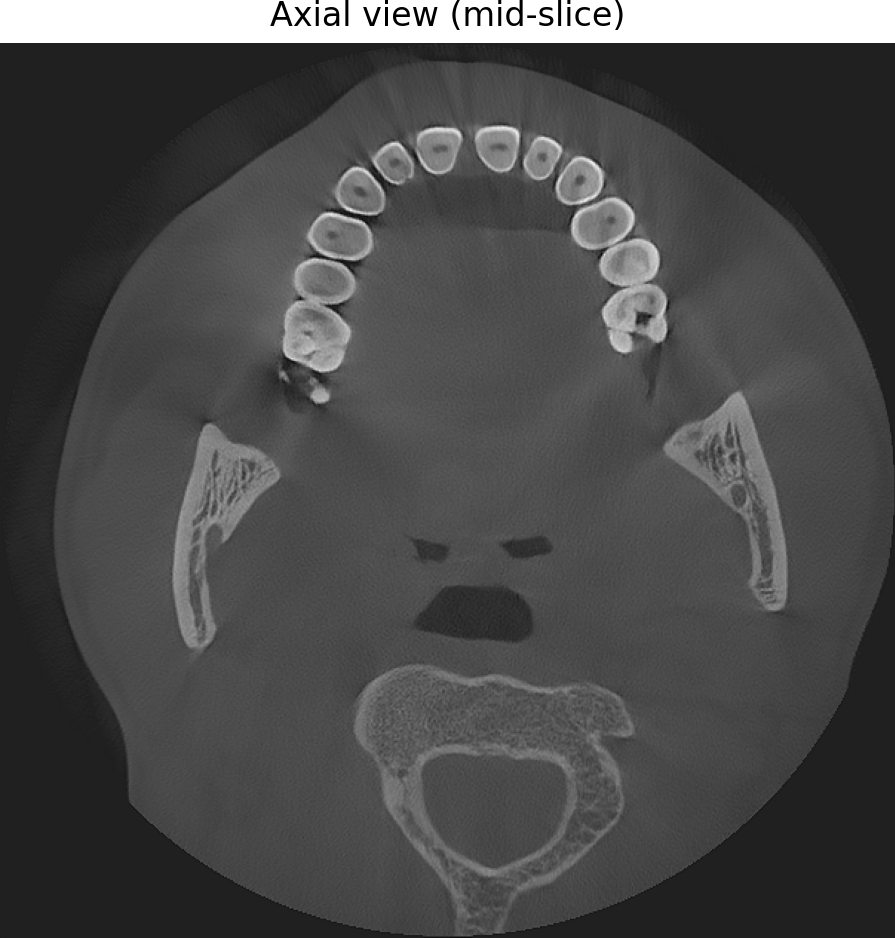
\includegraphics[width=0.10\textwidth]{../assets/cbctDifferentView/axial.png} &
        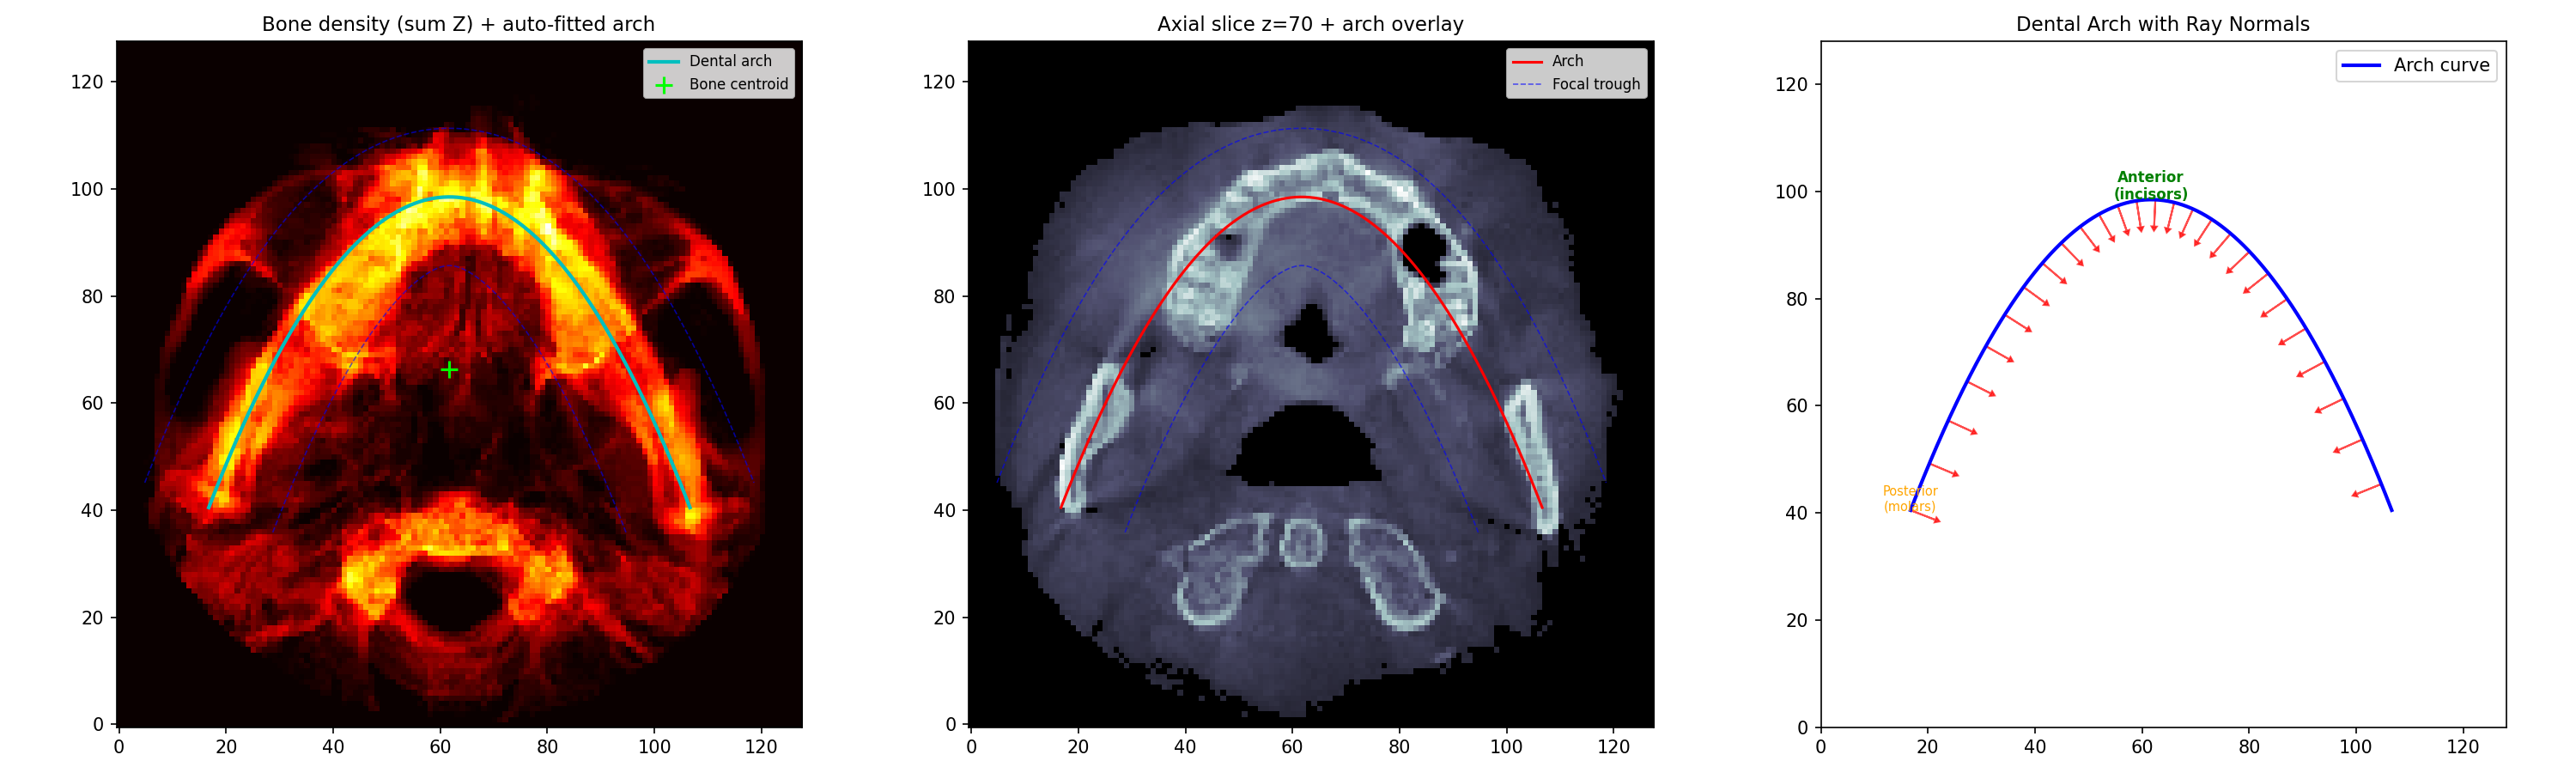
\includegraphics[width=0.10\textwidth]{../project/output/dental_arch_geometry.png} &
        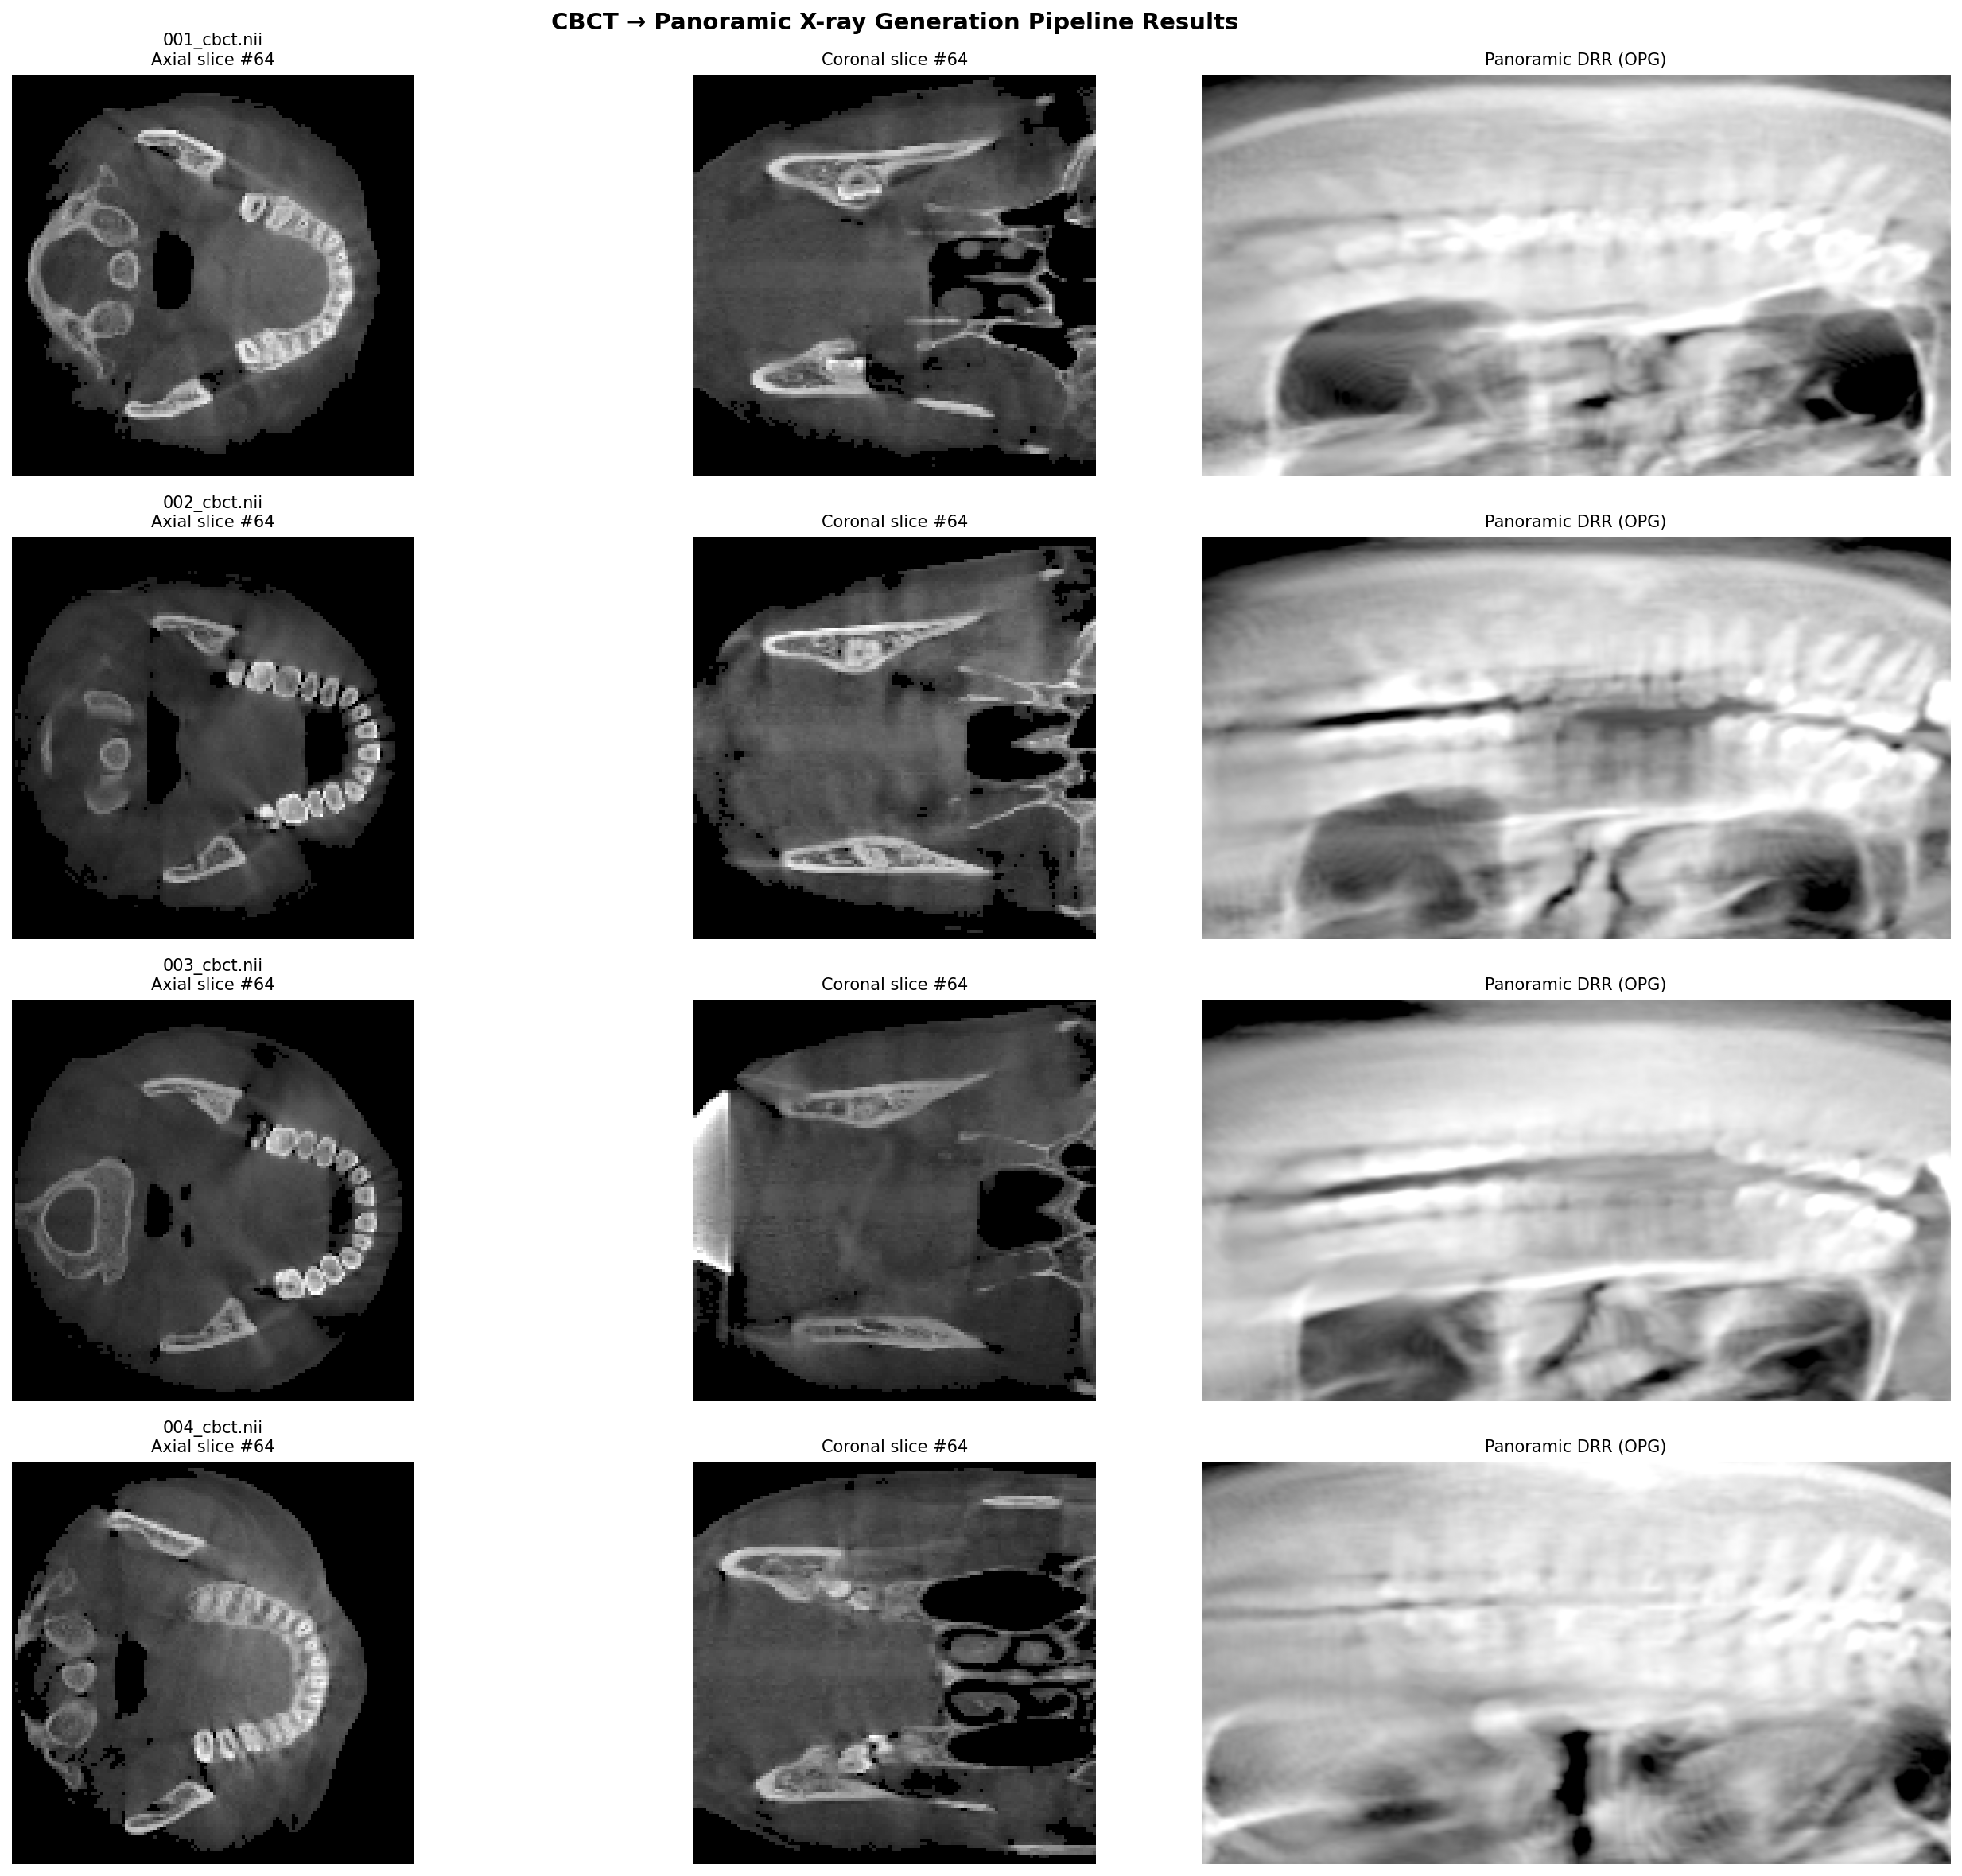
\includegraphics[width=0.10\textwidth]{../project/output/cbct_to_panoramic_comparison.png} &
        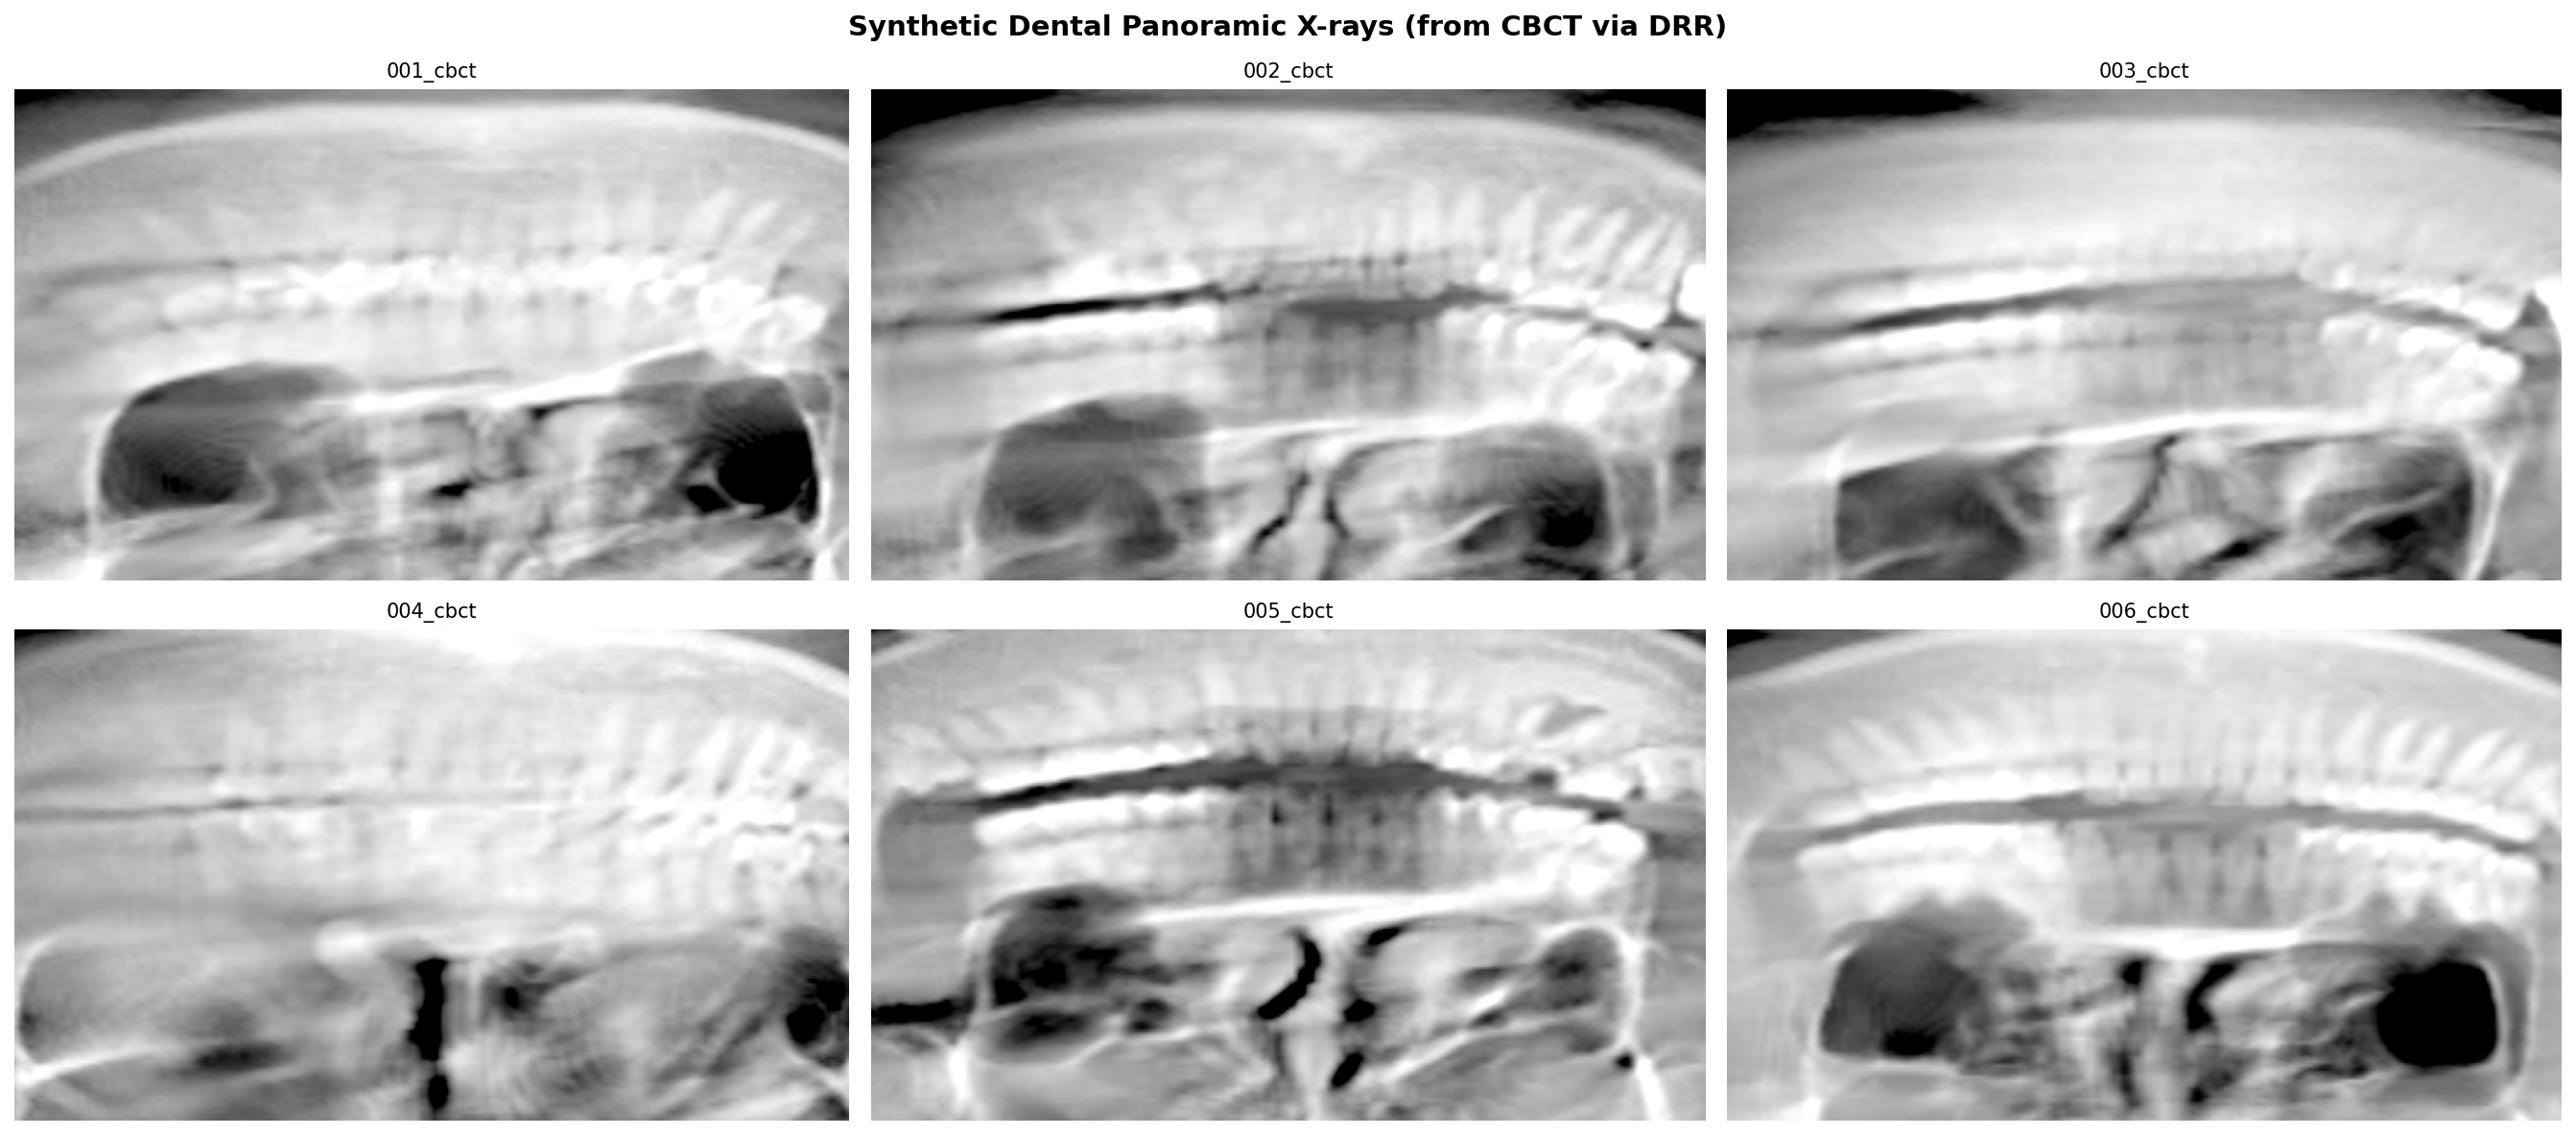
\includegraphics[width=0.10\textwidth]{../project/output/panoramic_grid.png} &
        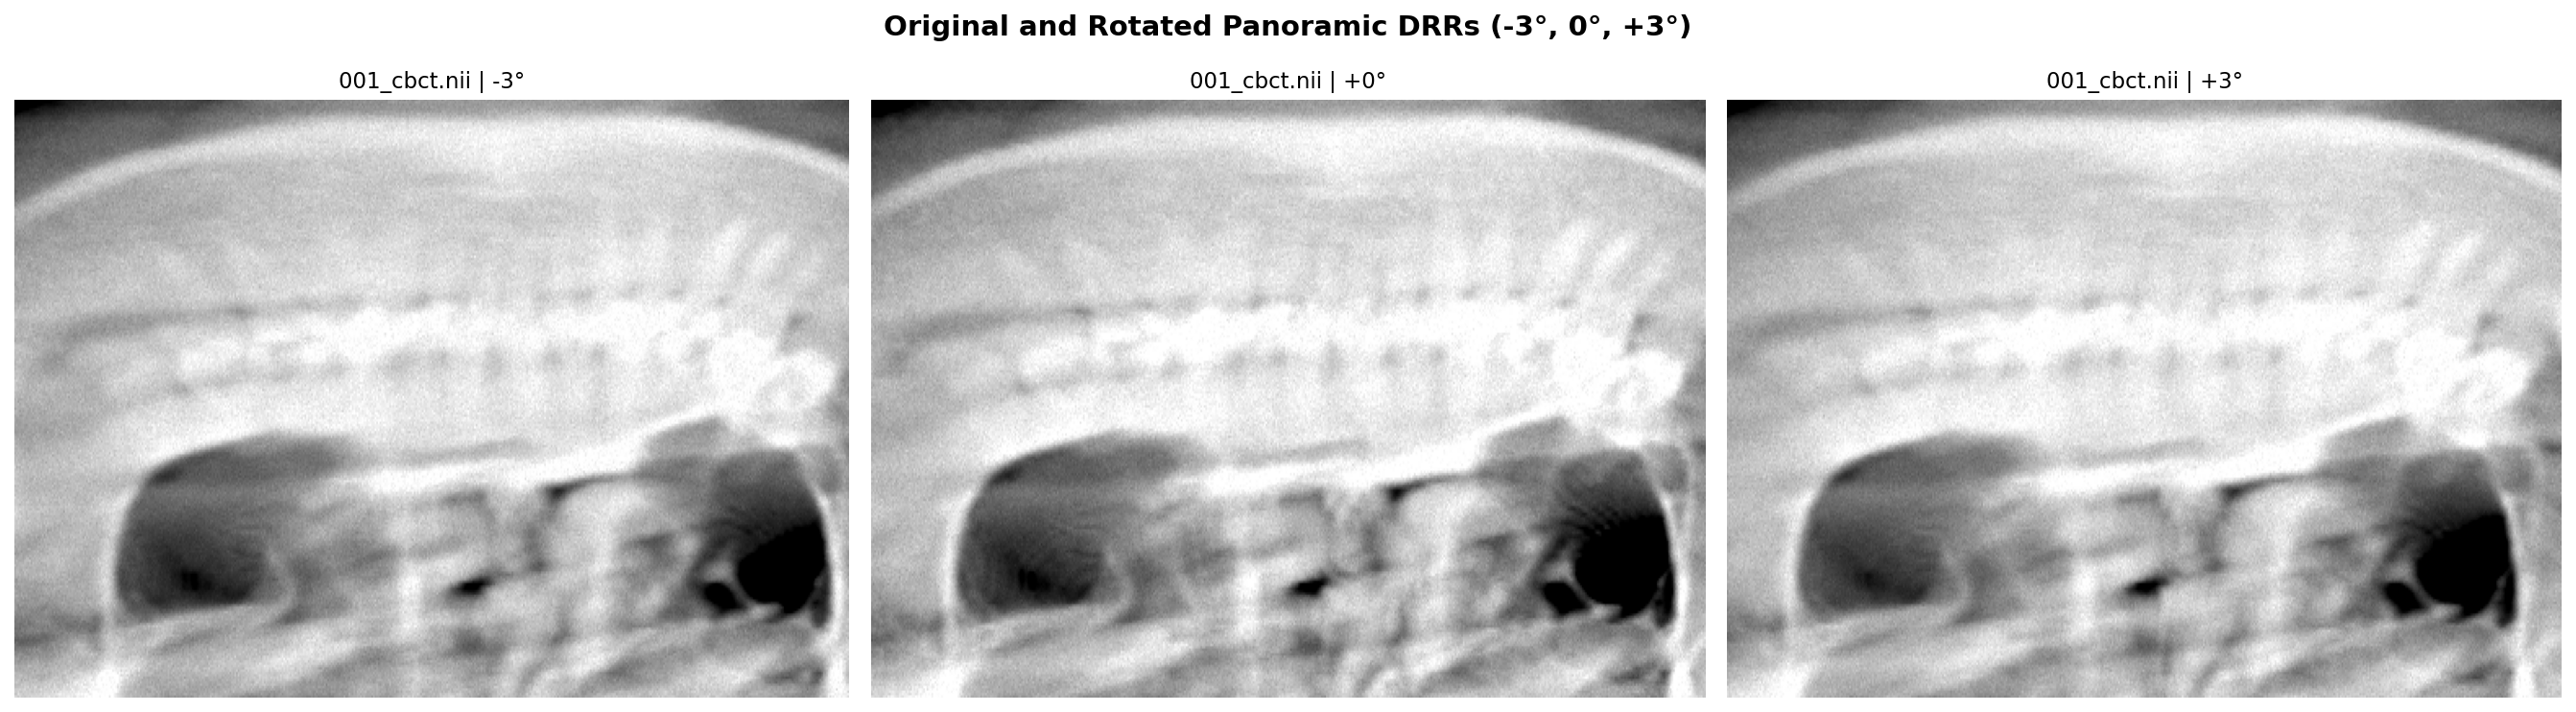
\includegraphics[width=0.10\textwidth]{../project/output/rotation_comparison_minus3_0_plus3.png} &
        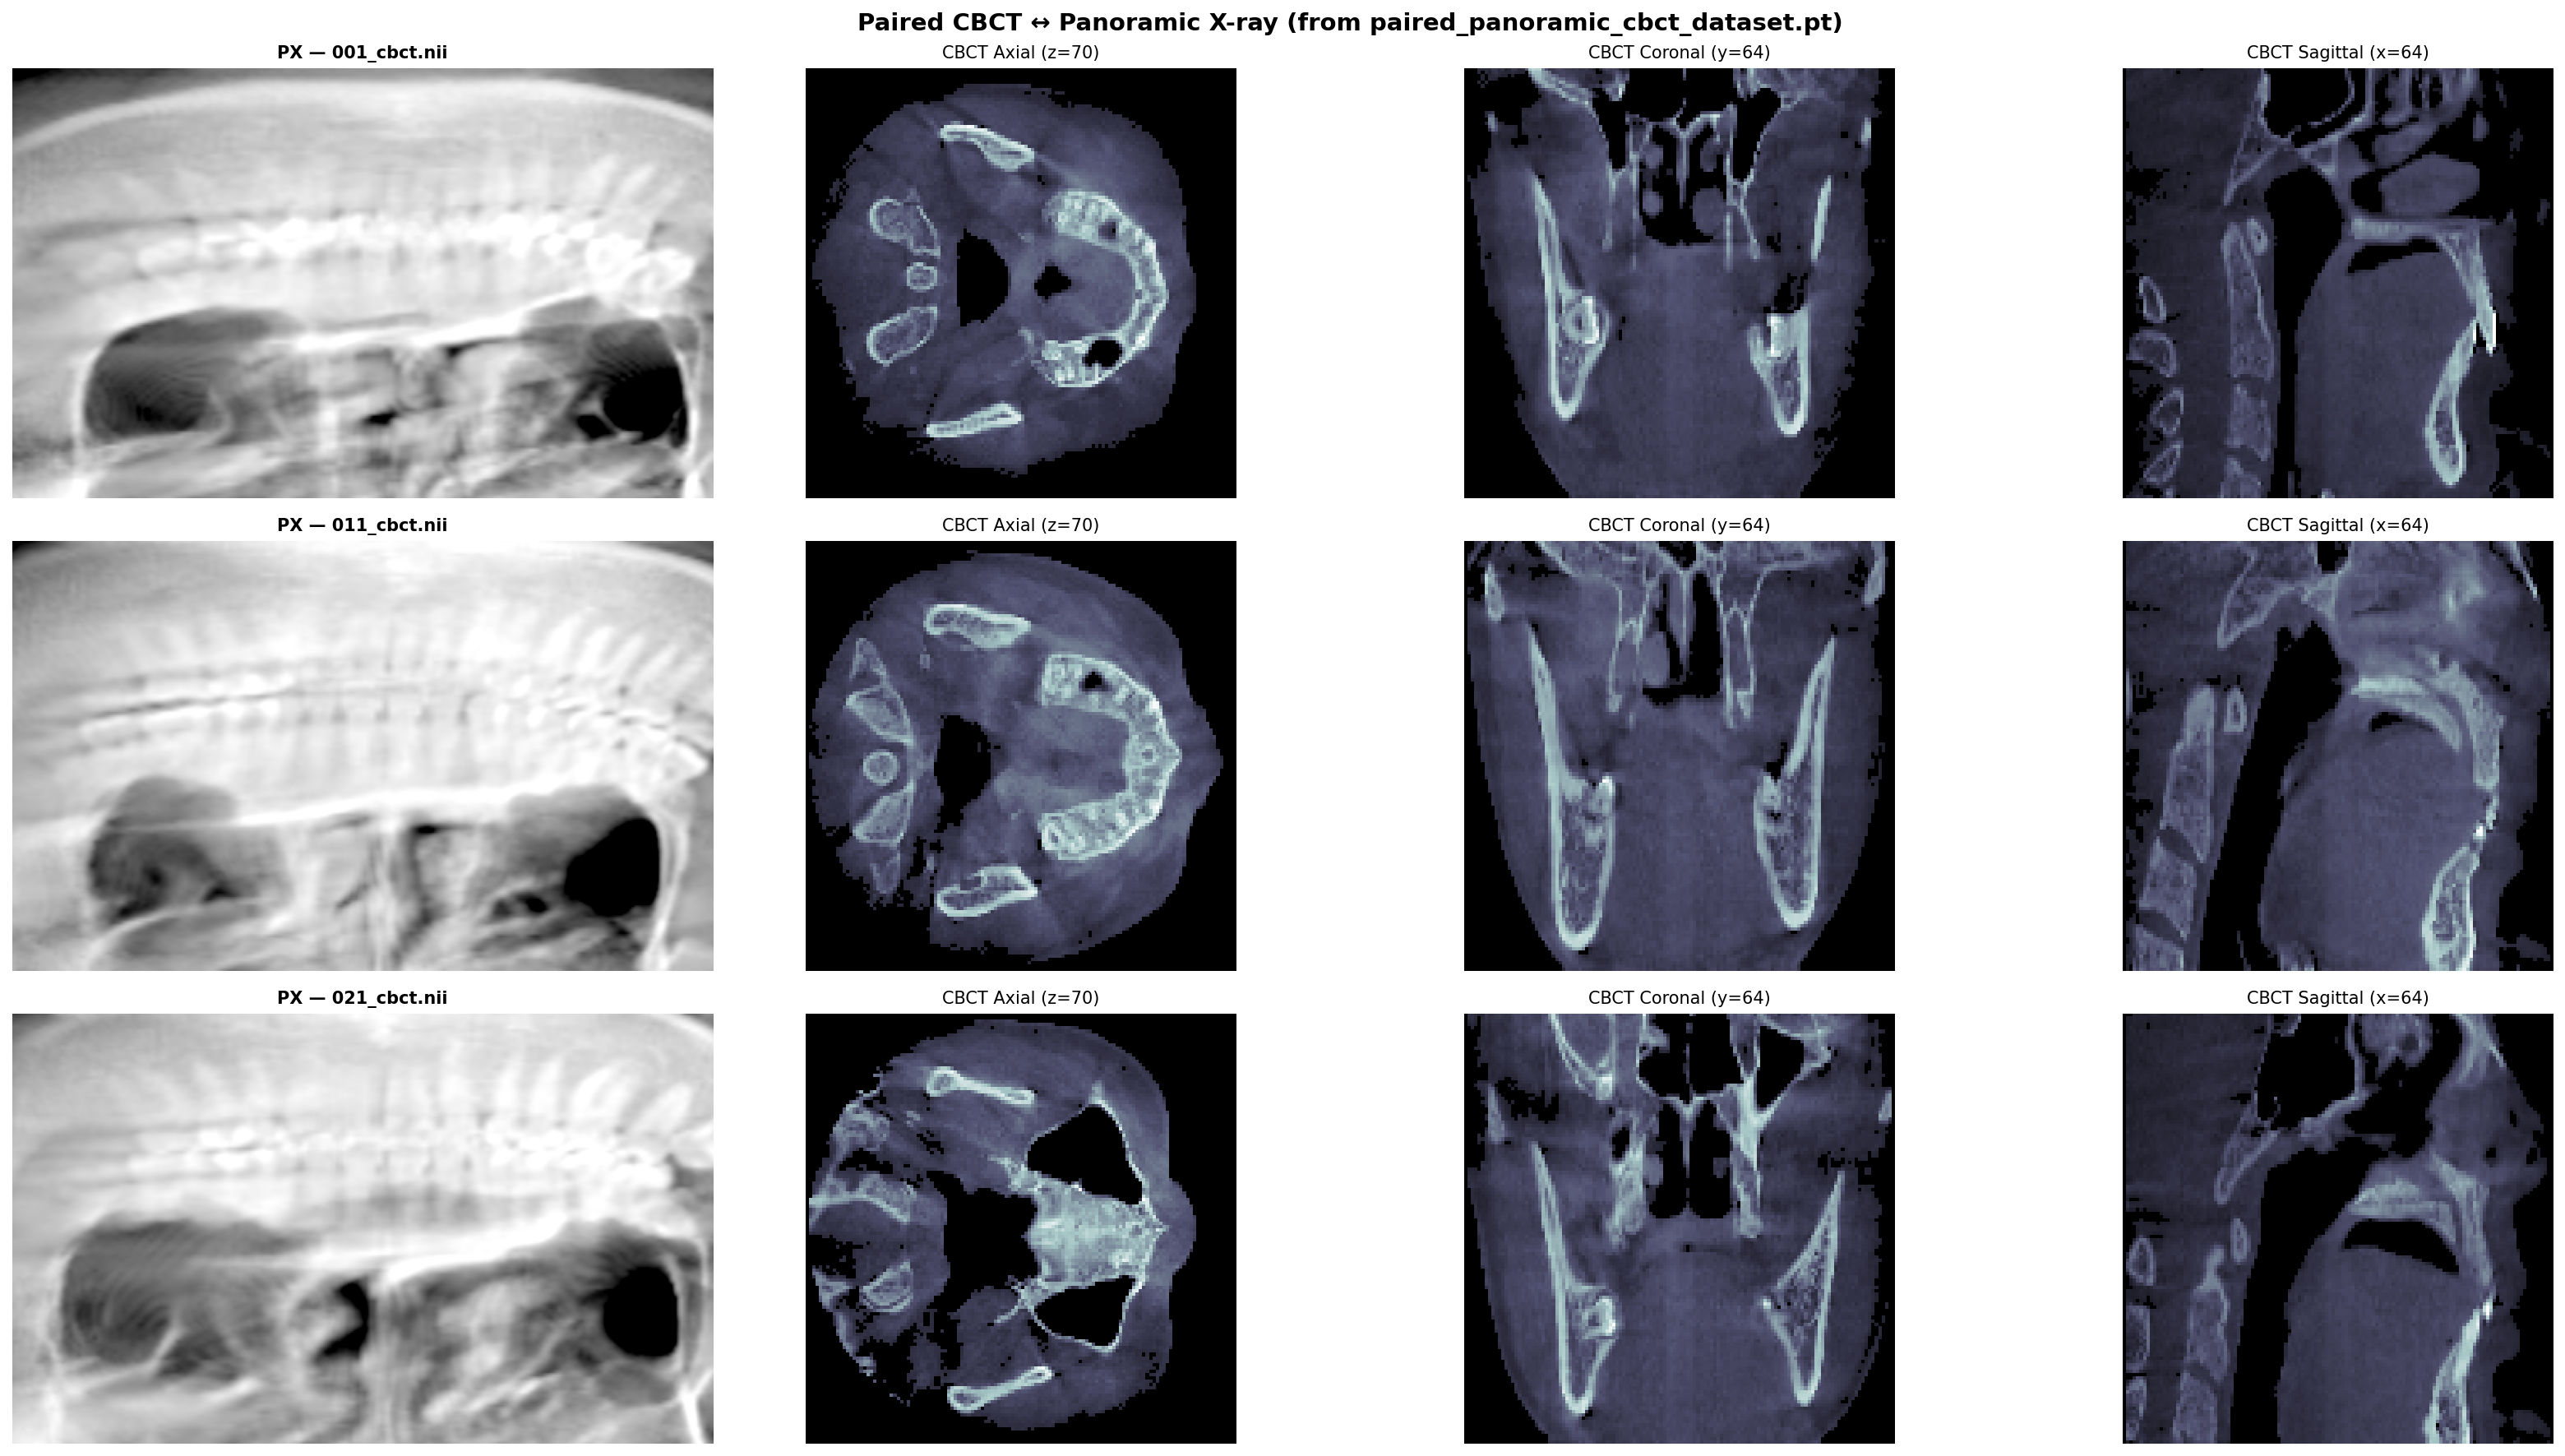
\includegraphics[width=0.10\textwidth]{../project/output/paired_cbct_px_samples.png} &
        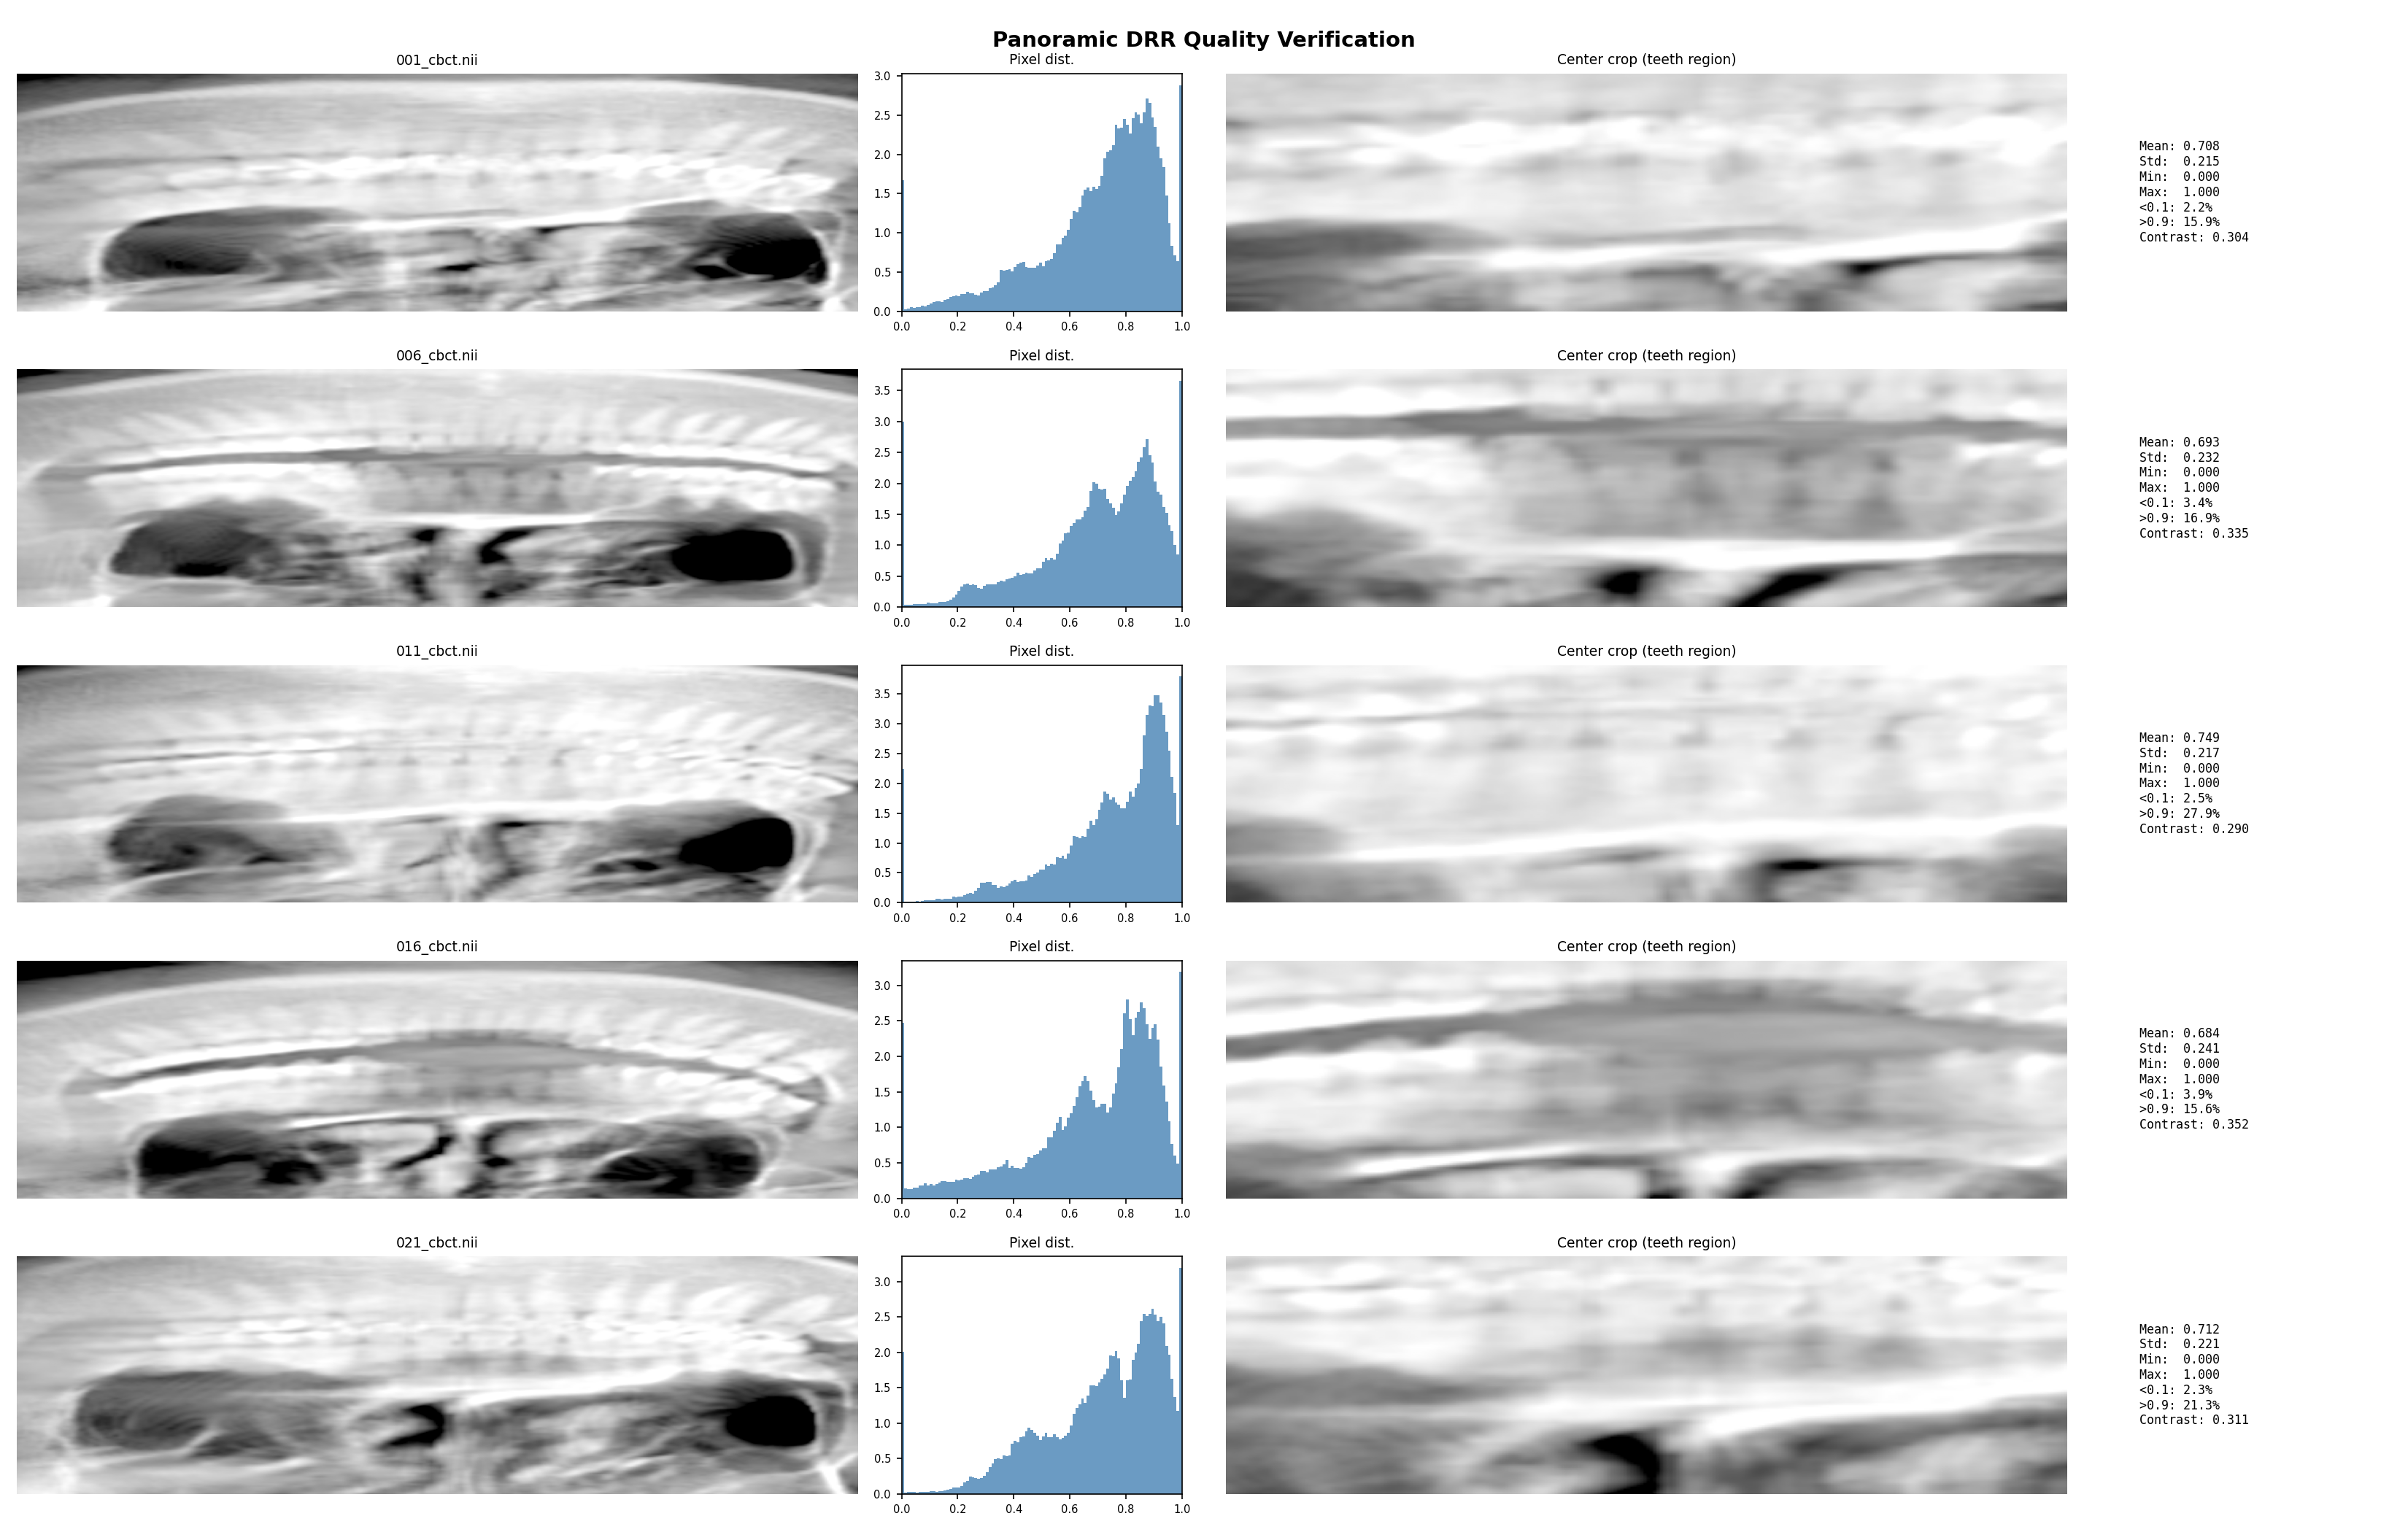
\includegraphics[width=0.10\textwidth]{../project/output/quality_verification.png} &
        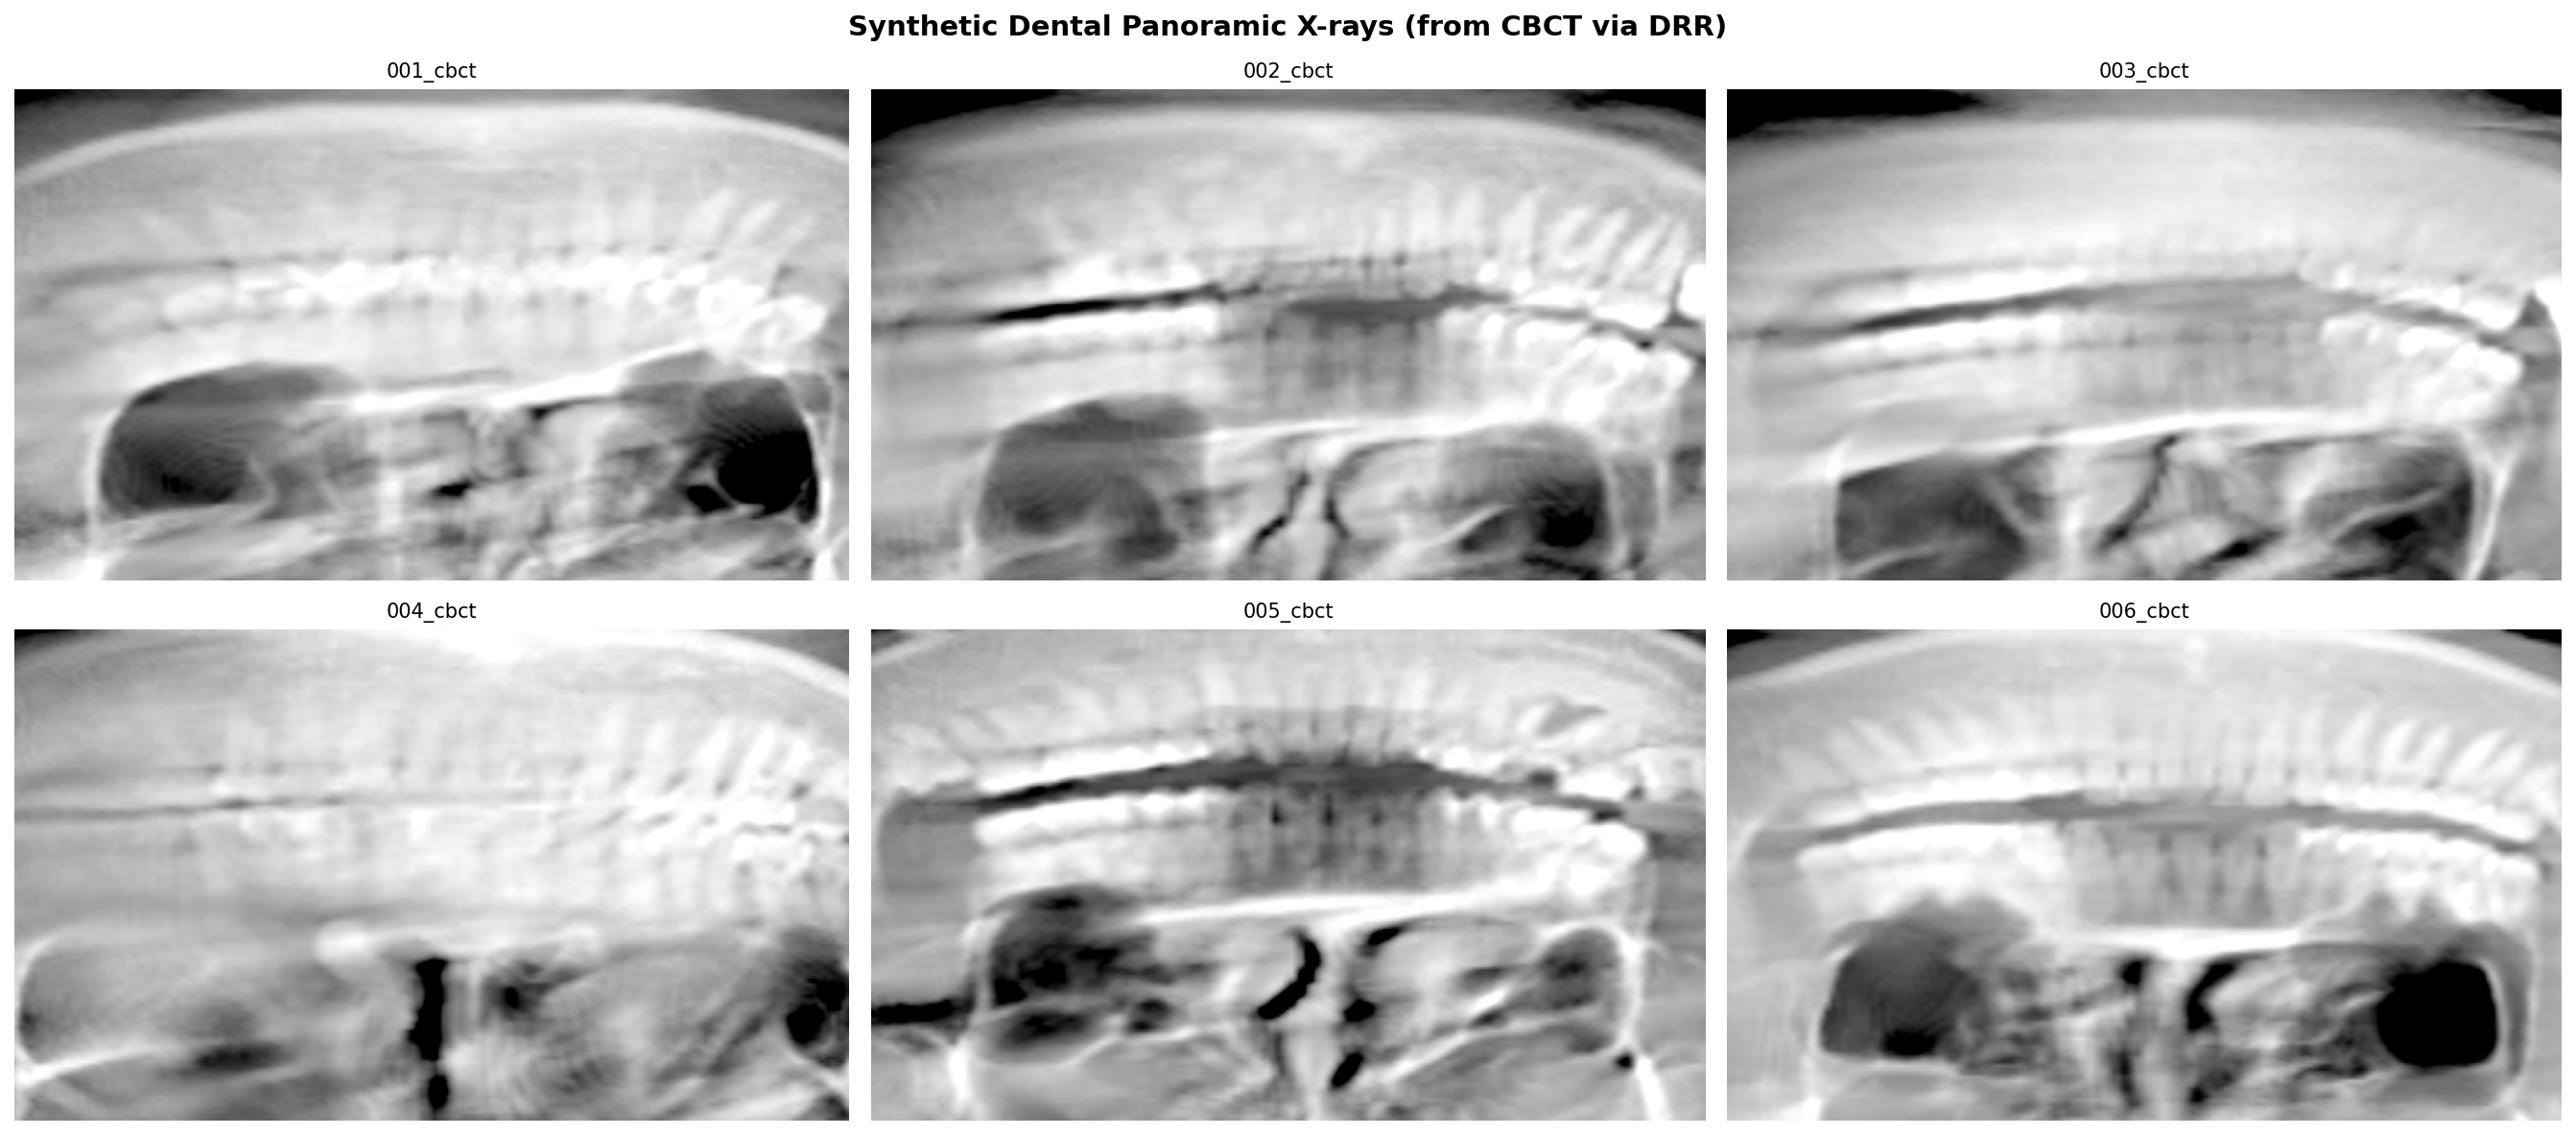
\includegraphics[width=0.10\textwidth]{../project/output/panoramic_grid.png} \\
        Input & Prep & Arch & DRR & PX & Aug & Pair & Eval & Output
    \end{tabular}
    \caption{CBCT volume processing flow used in this work}
    \label{fig:latest-method-architecture}
\end{figure}
\end{frame}

\begin{frame}{Ray Tracing on Curved Dental Arch}
\small
\begin{columns}[T,onlytextwidth]
    \begin{column}{0.56\textwidth}
        \begin{itemize}
            \item The panoramic trajectory is not planar; a \textbf{U-shaped dental arch} is estimated from high-density bone voxels.
            \item At each arch location, \textbf{normal vectors} are computed and rays are cast through a finite \textbf{focal trough depth}.
            \item Along each ray, attenuation coefficients $\mu$ are sampled by trilinear interpolation and integrated:
            \[
                \mathcal{I}(u,v)=\sum_{k=1}^{D} \mu_k \cdot \Delta l
            \]
            \item Post-processing (windowing, gamma correction, local contrast enhancement) improves radiographic realism.
        \end{itemize}
    \end{column}
    \begin{column}{0.44\textwidth}
        \begin{figure}
            \centering
            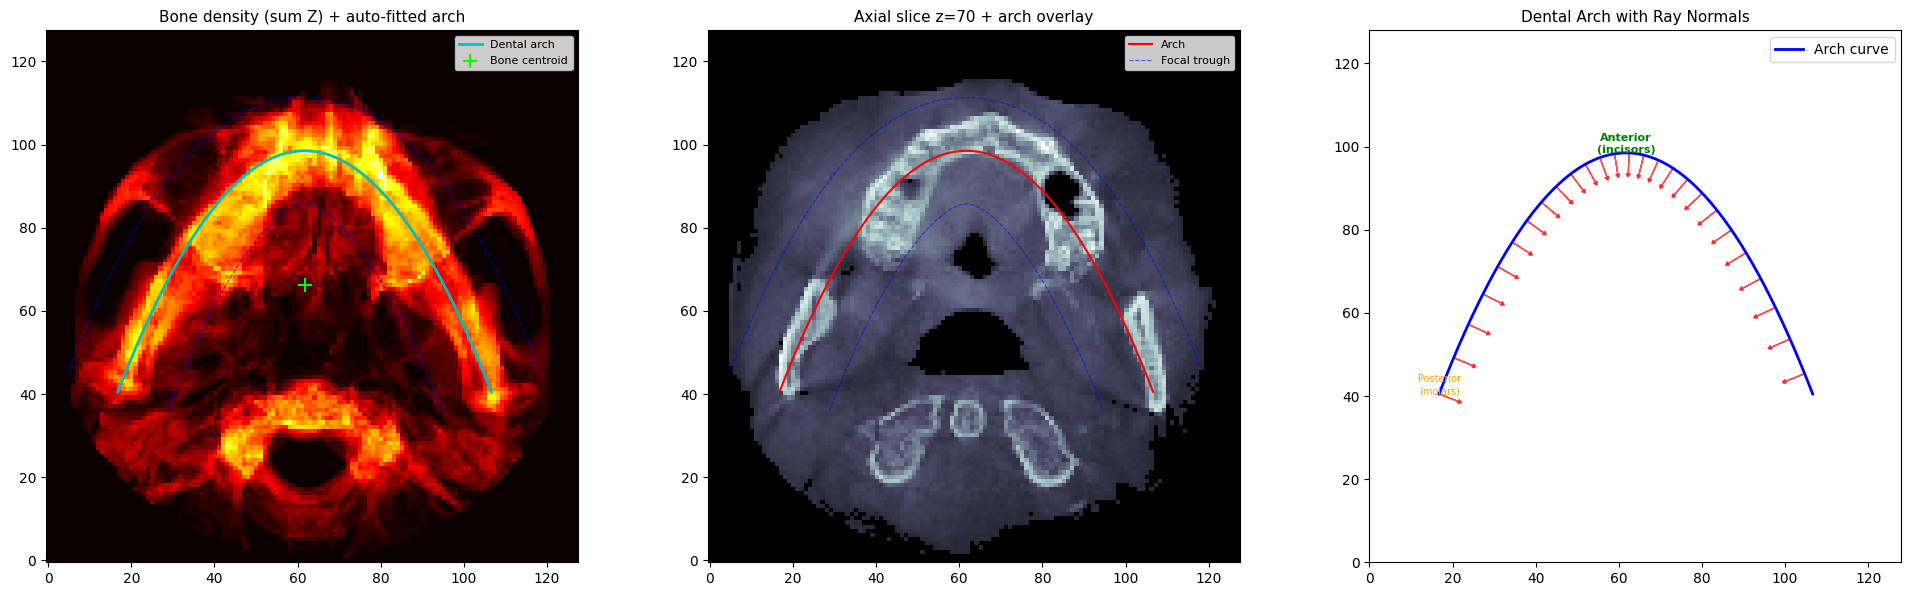
\includegraphics[width=\textwidth]{ray_tracing_result.png}
            \caption{Ray tracing result on curved dental arch}
            \label{fig:ray-tracing-result}
        \end{figure}
    \end{column}
\end{columns}
\end{frame}

% \begin{frame}{Curved-Arch Ray Tracing Illustration}
% \begin{figure}
%     \centering
%     \includegraphics[width=0.75\textwidth]{Explained_ray_tracing2.png}
%     \caption{Explained curved-arch ray tracing through the focal trough for panoramic DRR generation}
%     \label{fig:ray-tracing-latest}
% \end{figure}
% \end{frame}

\begin{frame}{Ray Tracing Equations (DRR Formulation)}
\small
\begin{columns}[T,onlytextwidth]
    \begin{column}{0.58\textwidth}
        \textbf{1) Beer-Lambert attenuation along a ray}
        \[
        I(u,v)=I_0\exp\left(-\int_{\mathcal{L}(u,v)} \mu(\mathbf{x})\,d\ell\right)
        \]

        \textbf{2) Discrete approximation used in implementation}
        \[
        A(u,v)\approx\sum_{k=1}^{D} \mu_k\,\Delta \ell
        \]
        where $\mu_k$ is trilinearly sampled

        \textbf{3) Pixel formation for panoramic DRR}
        \[
        I(u,v)=\exp\left(-A(u,v)\right)
        \]
      $A(u,v)$ is further windowed and contrast-enhanced to match panoramic appearance.
    \end{column}
    \begin{column}{0.42\textwidth}
        \begin{figure}
            \centering
            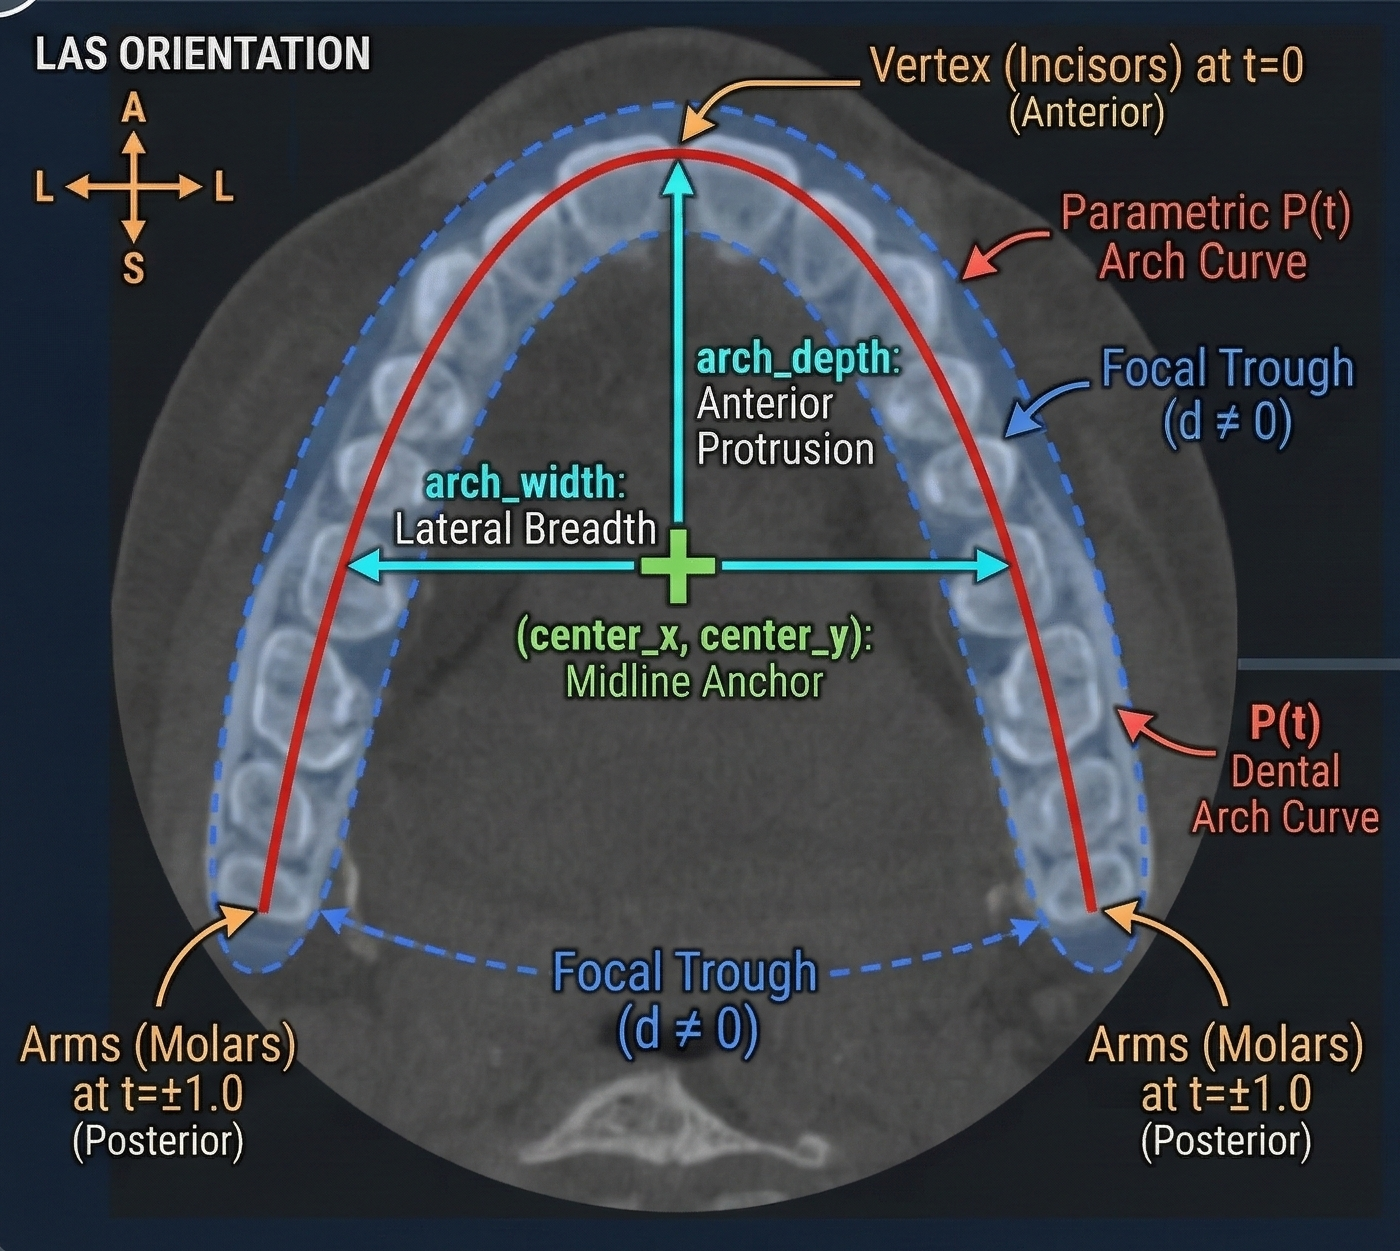
\includegraphics[width=\textwidth]{Explained_Ray_tracing.png}
            \caption{Equation-level view of curved focal-trough ray tracing}
            \label{fig:ray-tracing-equations}
        \end{figure}
    \end{column}
\end{columns}
\end{frame}

% \begin{frame}{Implementation Steps}
% \small
% \begin{enumerate}
%     \item Load all CBCT files and extract shape, spacing, intensity statistics.
%     \item Resample to isotropic spacing and resize to a fixed 3D cube.
%     \item Convert HU-like values to attenuation map $\mu$ for physically meaningful projection.
%     \item Detect dental arch parameters from tooth-level bone regions.
%     \item Build curved focal-trough sampling grid and generate panoramic DRRs.
%     \item Create augmented multi-view panoramics (small rotations, noise, intensity jitter).
%     \item Build paired PyTorch dataset \texttt{(panoramic, cbct, metadata)}.
%     \item Evaluate quality with combined loss and summary metrics.
% \end{enumerate}
% \end{frame}

\begin{frame}{Results}
\small
\begin{columns}[T,onlytextwidth]
    \begin{column}{0.55\textwidth}
        \textbf{Generated artifacts from the methodology}
        \begin{itemize}
            \item Synthetic panoramic PNGs for each CBCT volume.
            \item Augmented panoramic dataset for robustness experiments.
            \item Paired dataset file: \texttt{paired\_panoramic\_cbct\_dataset.pt}.
            \item Visual diagnostics: arch geometry, panoramic grid, quality verification plots.
        \end{itemize}

        \vspace{0.2cm}
        \textbf{Quantitative checks}
        \begin{itemize}
            \item Pixel losses: L1=0.03146
            \item Structural metric: SSIM=0.76
            \item Signal fidelity: PSNR=20.76db
        \end{itemize}
    \end{column}
    \begin{column}{0.45\textwidth}
        \begin{figure}
            \centering
            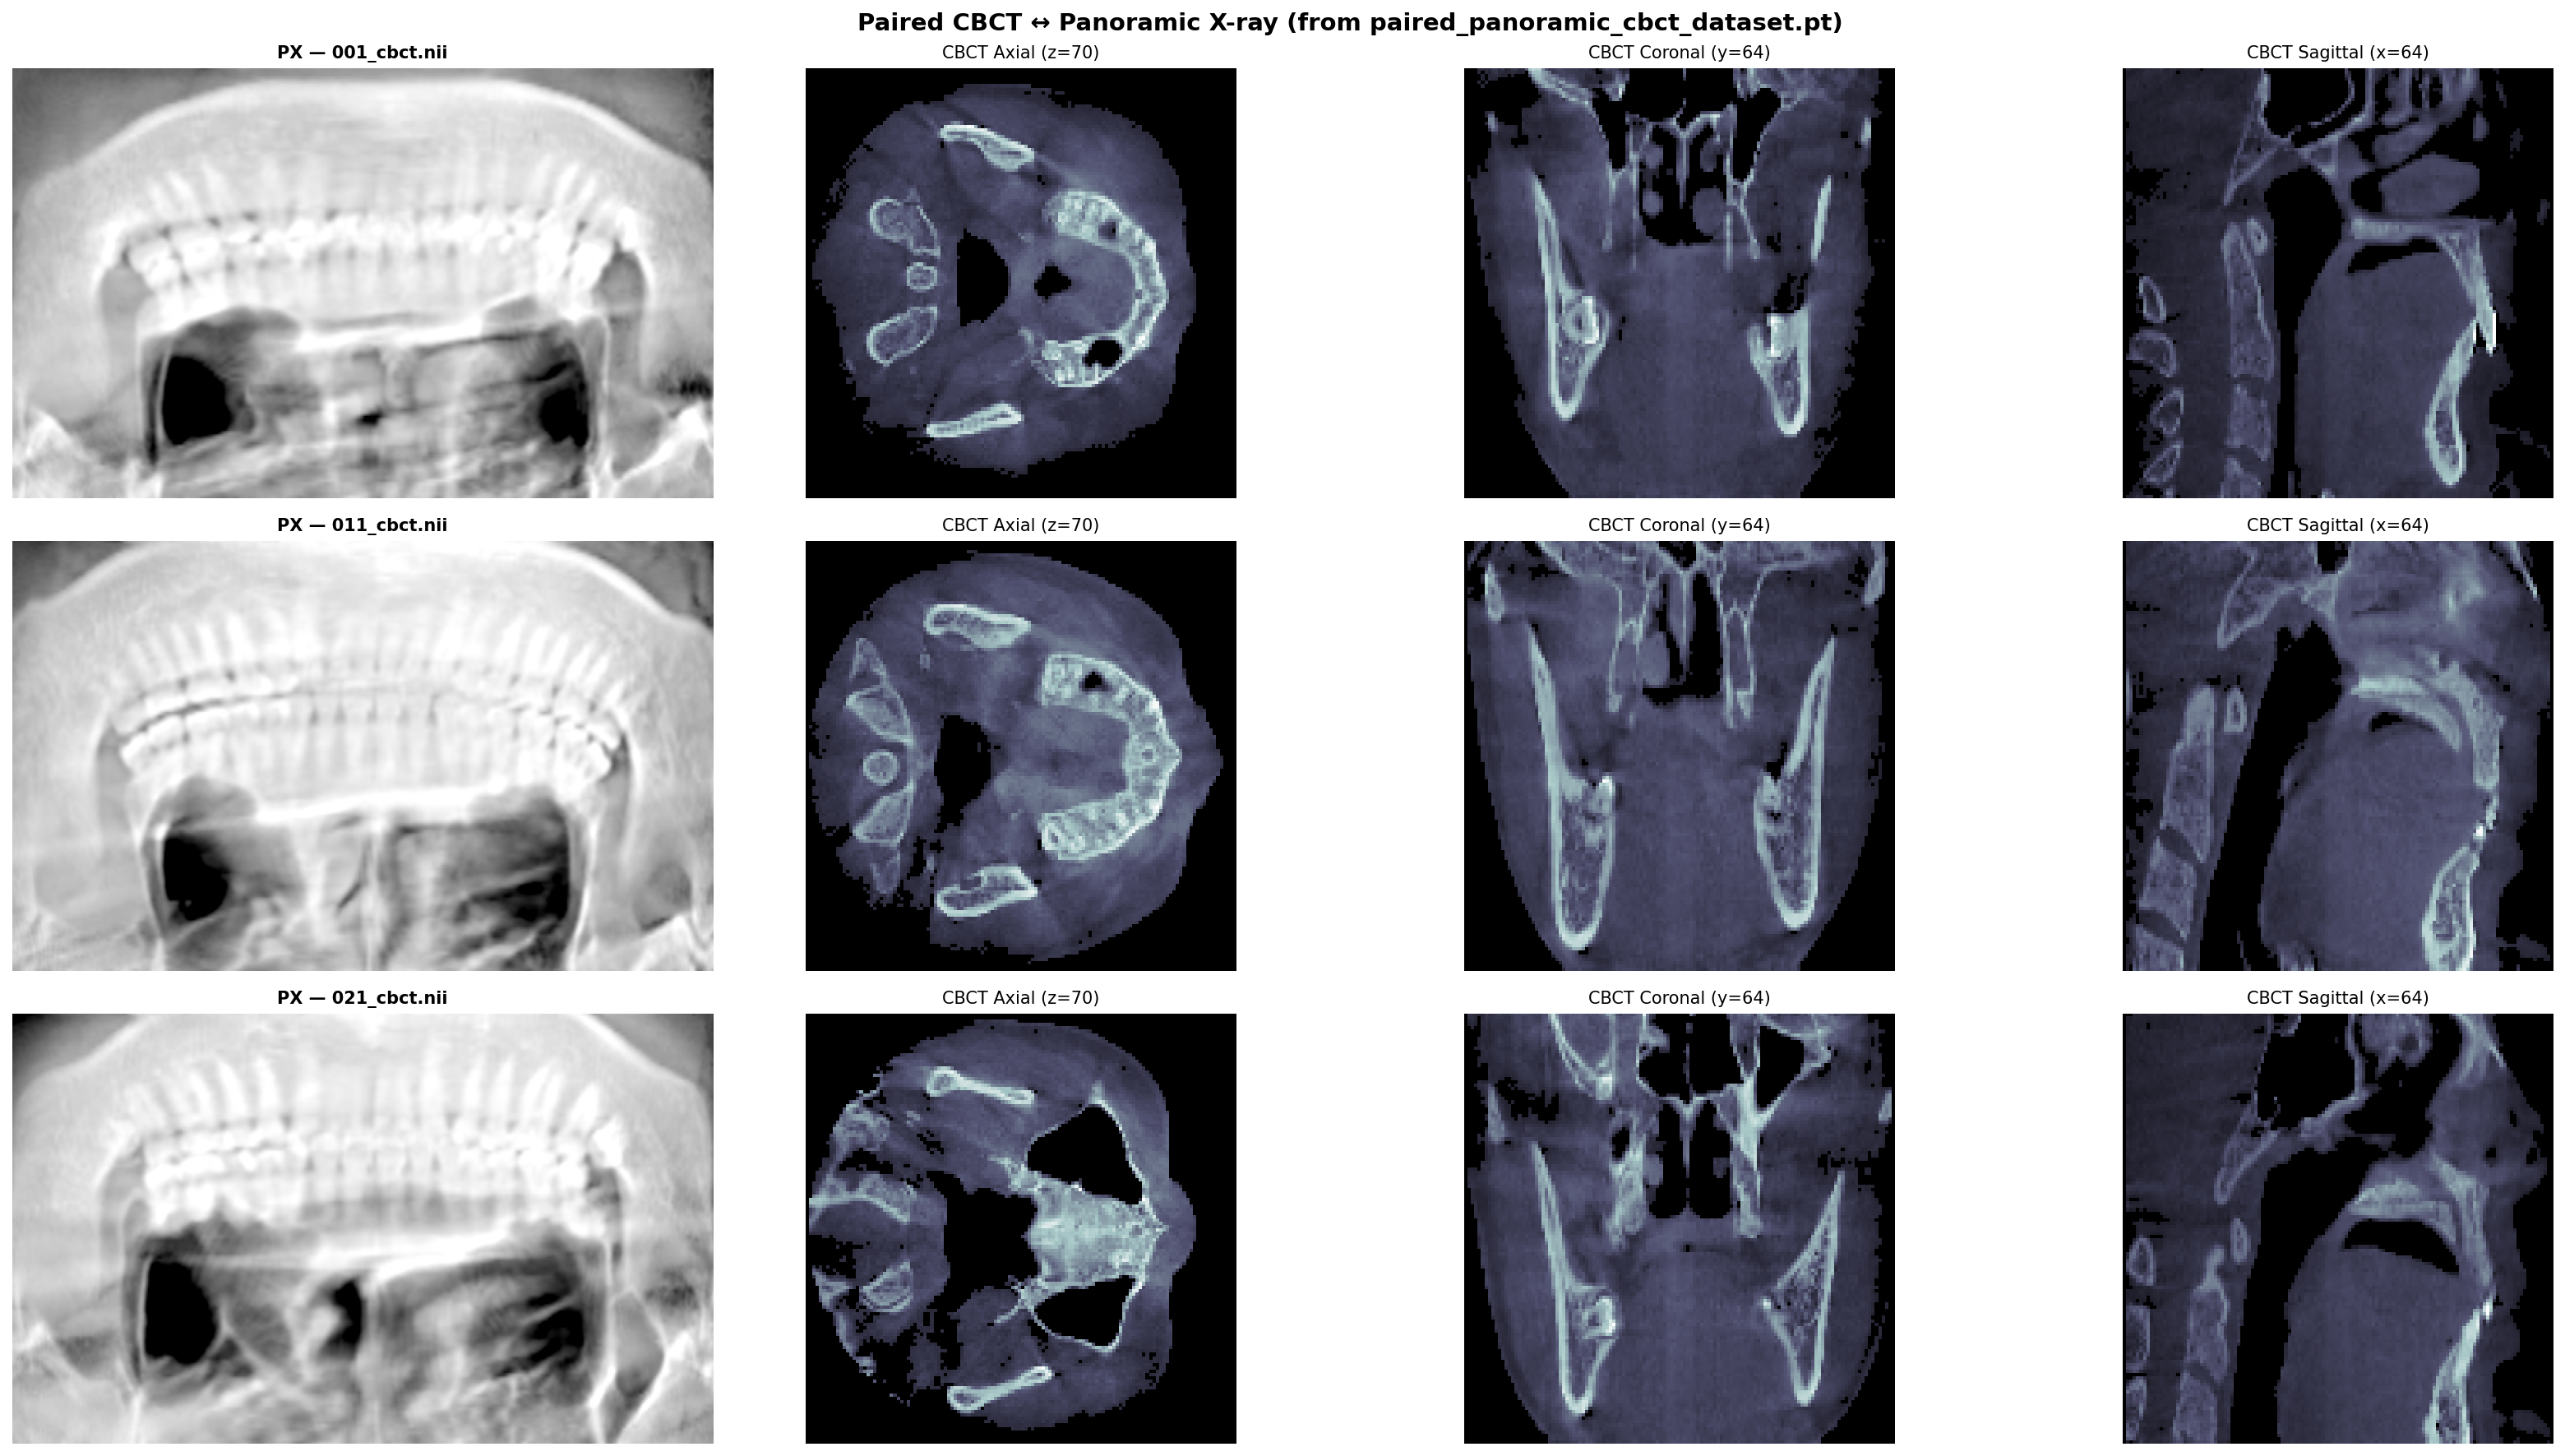
\includegraphics[width=\textwidth]{paired_cbct_px_samples.png}
            \caption{Example paired CBCT slices and generated panoramic image}
            \label{fig:method-outputs-paired}
        \end{figure}
    \end{column}
\end{columns}
\end{frame}

\section{Conclusion}

\begin{frame}{Results}
\small
\begin{columns}[T,onlytextwidth]
    \begin{column}{0.52\textwidth}
        \textbf{Pipeline-driven outputs}
        \begin{itemize}
            \item Processed \textbf{21 CBCT} volumes and generated synthetic panoramic DRRs.
            \item Saved one panoramic output per volume.
            \item Built augmented views using rotations \texttt{[-3, 0, +3]} (total \textbf{63} panoramic variants).
            \item Exported paired training artifact in a pytorch model file.
            \item Produced diagnostic figures for arch geometry and image quality verification.
        \end{itemize}
    \end{column}
    \begin{column}{0.48\textwidth}
        \begin{figure}
            \centering
            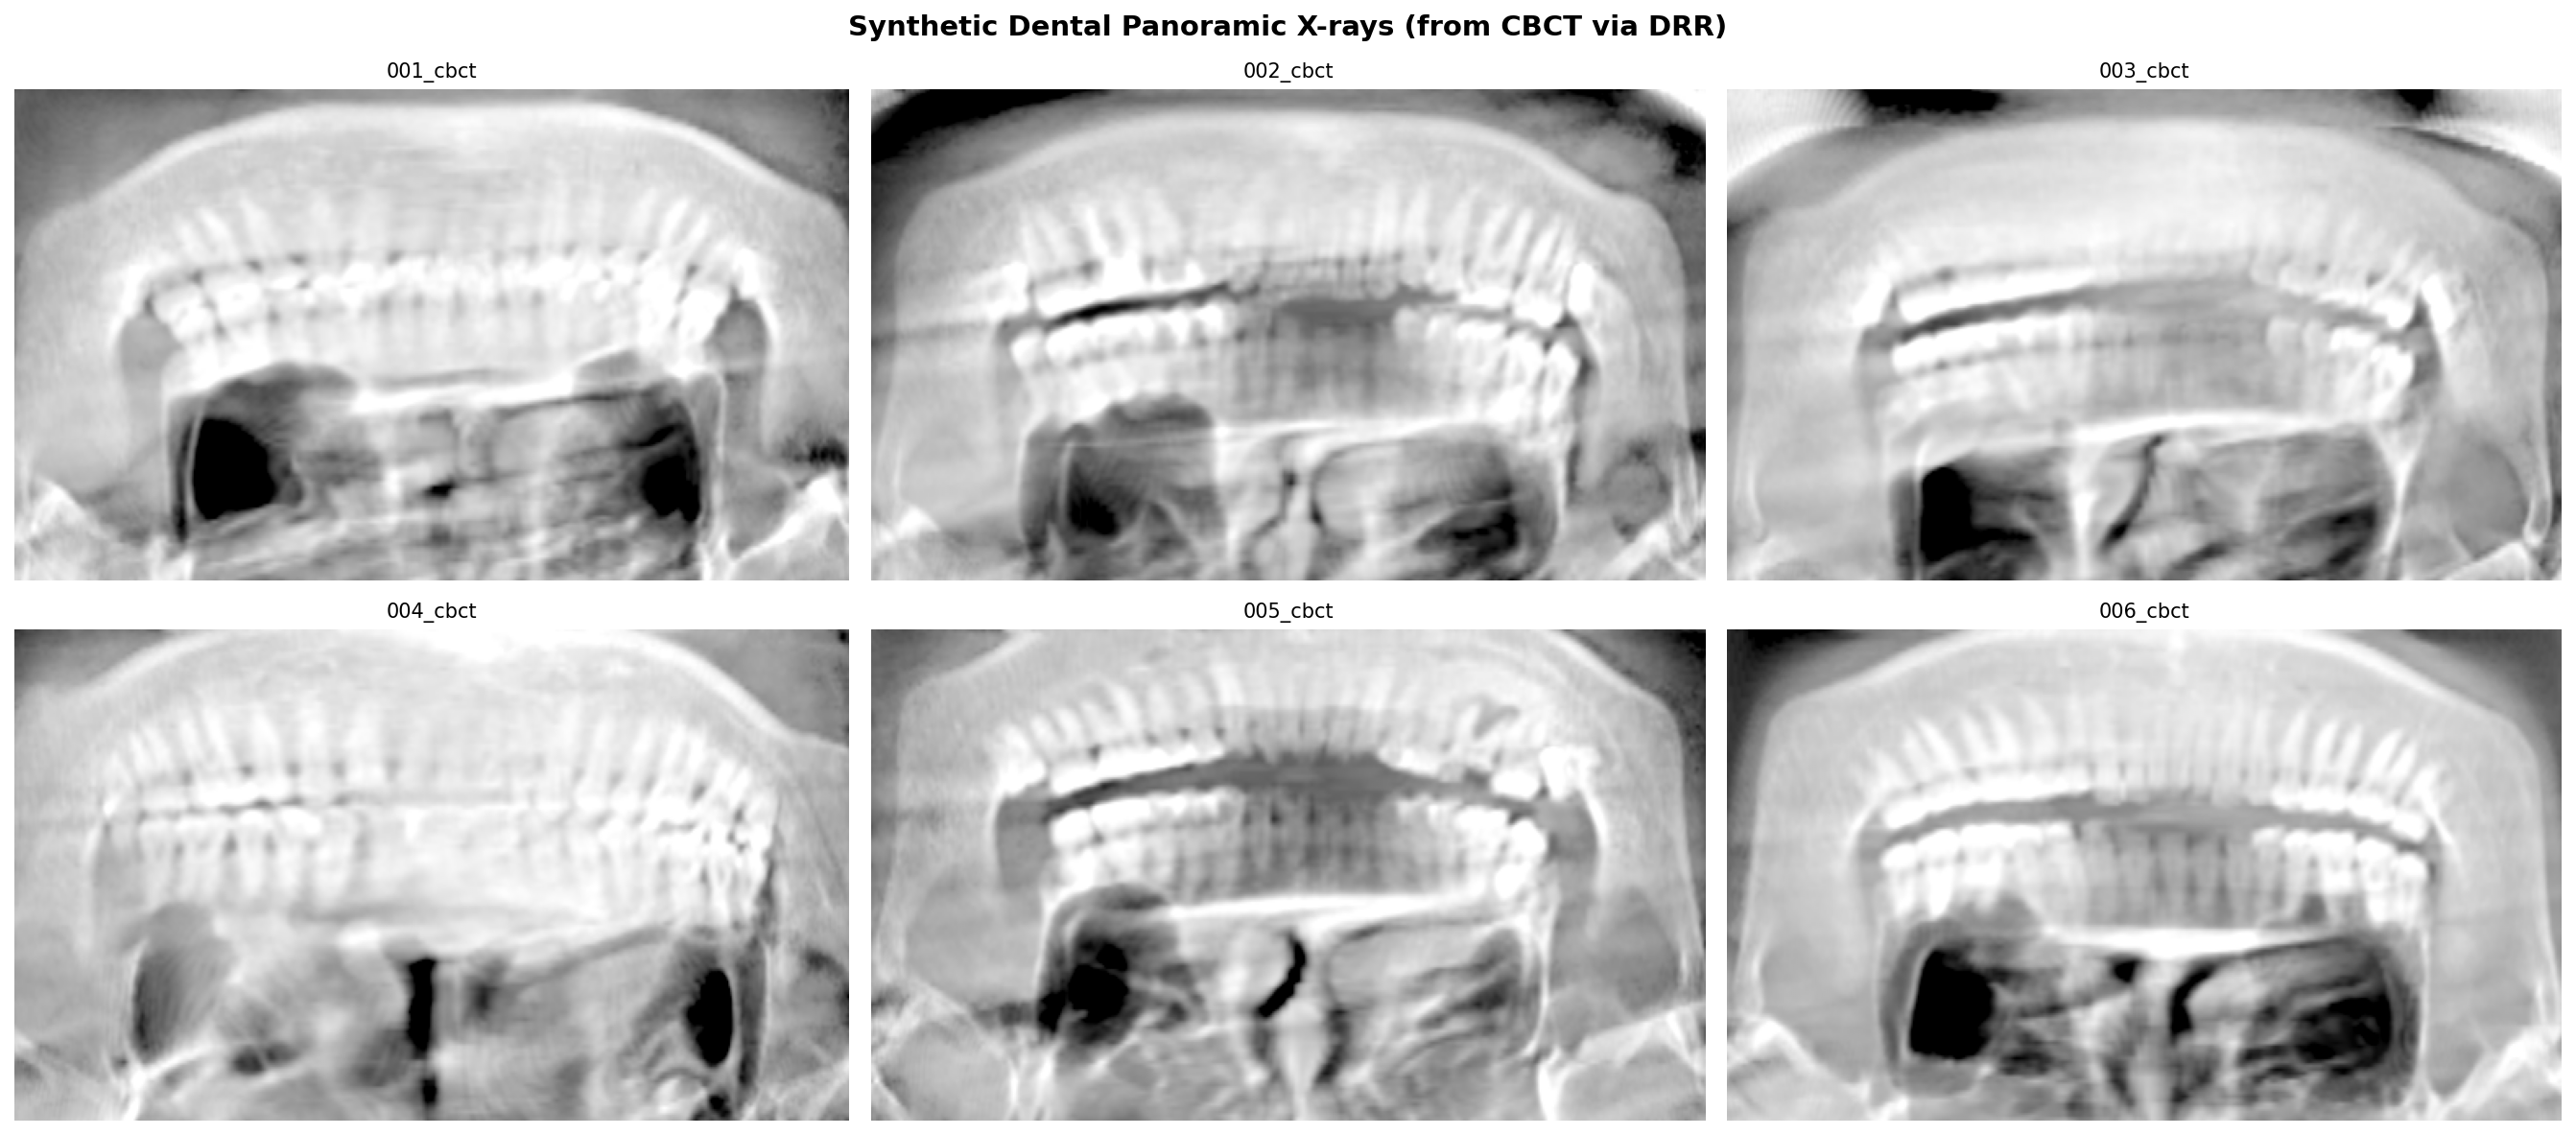
\includegraphics[width=\textwidth]{panoramic_grid.png}
            \caption{Grid of synthetic panoramic X-rays generated from CBCT volumes}
            \label{fig:results-panoramic-grid}
        \end{figure}
    \end{column}
\end{columns}

\end{frame}

\begin{frame}{Results: NeBLa vs Our Output Comparison}
\begin{figure}
    \centering
    \begin{tabular}{cc}
        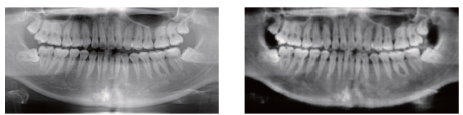
\includegraphics[width=0.47\textwidth]{nebla.png} &
        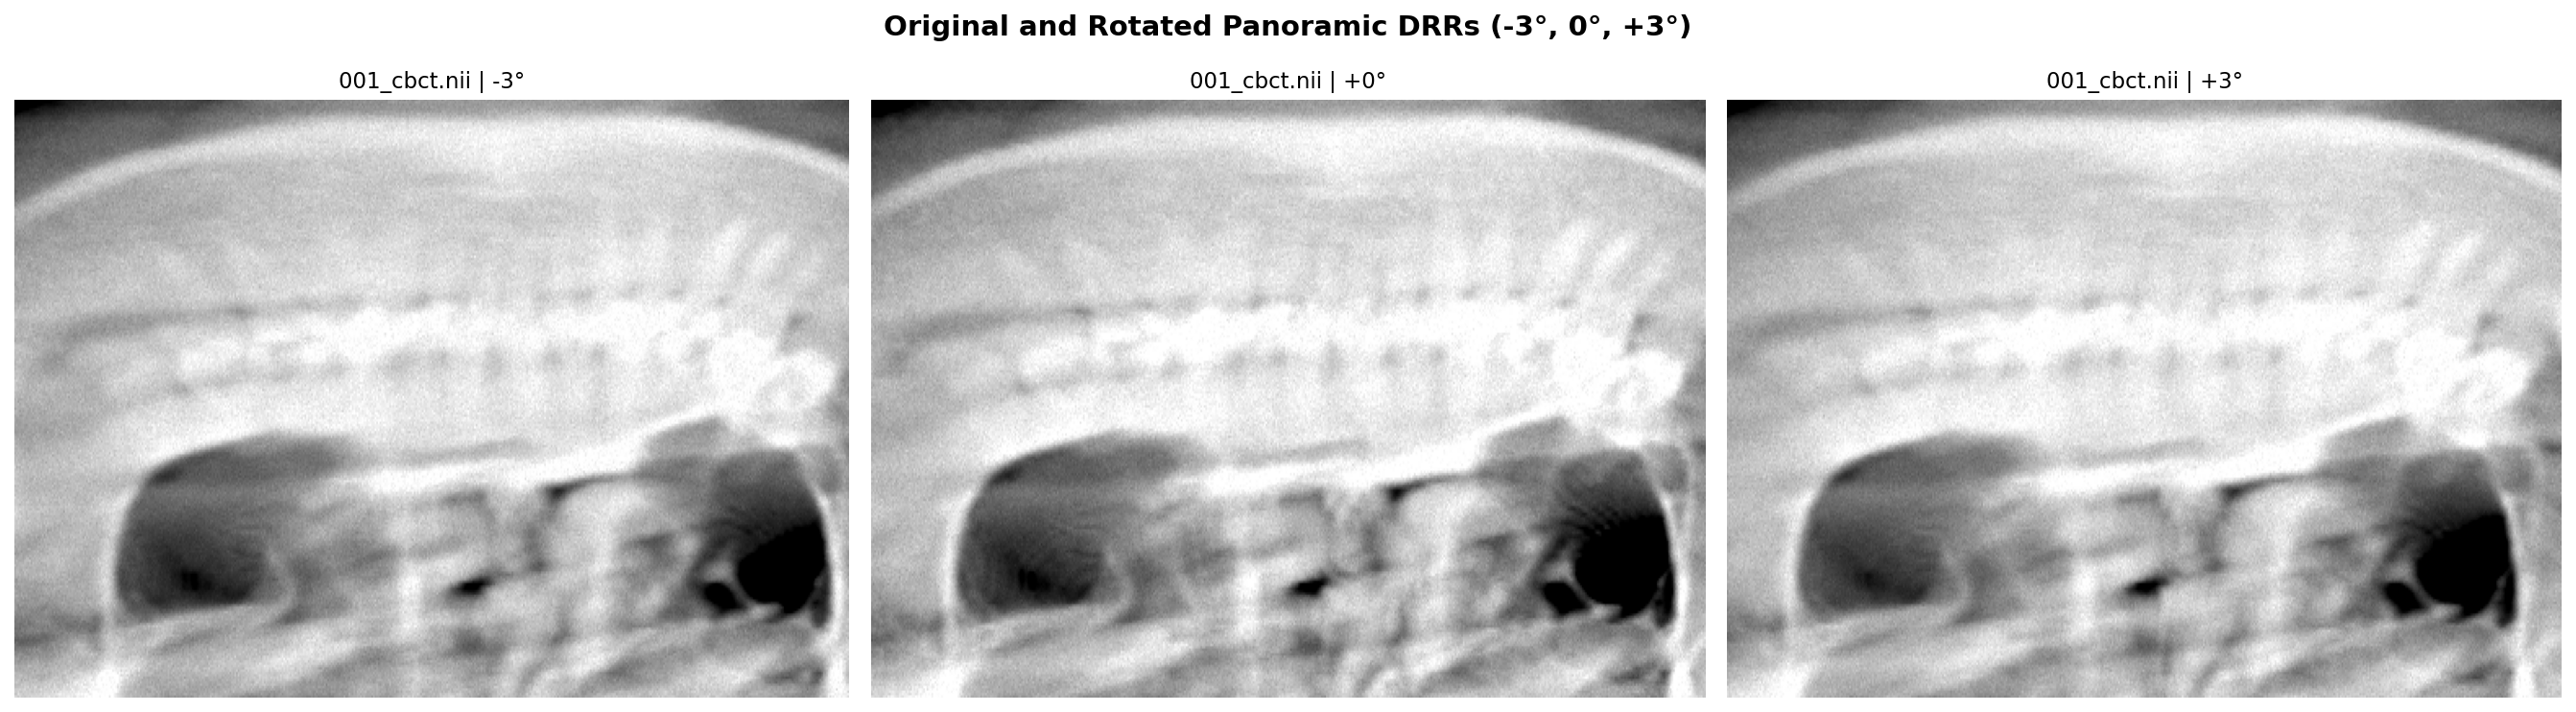
\includegraphics[width=0.47\textwidth]{../project/output/rotation_comparison_minus3_0_plus3.png} \\
        \footnotesize NeBLa Reference Output & \footnotesize Our Output ($-3^{\circ}, 0^{\circ}, +3^{\circ}$)
    \end{tabular}
    \\
    \vspace{0.2cm}
    \scriptsize
    \begin{tabular}{cc}
        \textbf{NeBLa:} PSNR = 19.89, SSIM = 0.79 & \textbf{Ours:} PSNR = 20.76, SSIM = 0.76
    \end{tabular}
    \caption{Comparison between NeBLa reference and our generated panoramic outputs}
    \label{fig:nebla-vs-ours-comparison}
\end{figure}
\end{frame}

\begin{frame}{Results: CBCT to Panoramic Visualization}
\begin{figure}
    \centering
    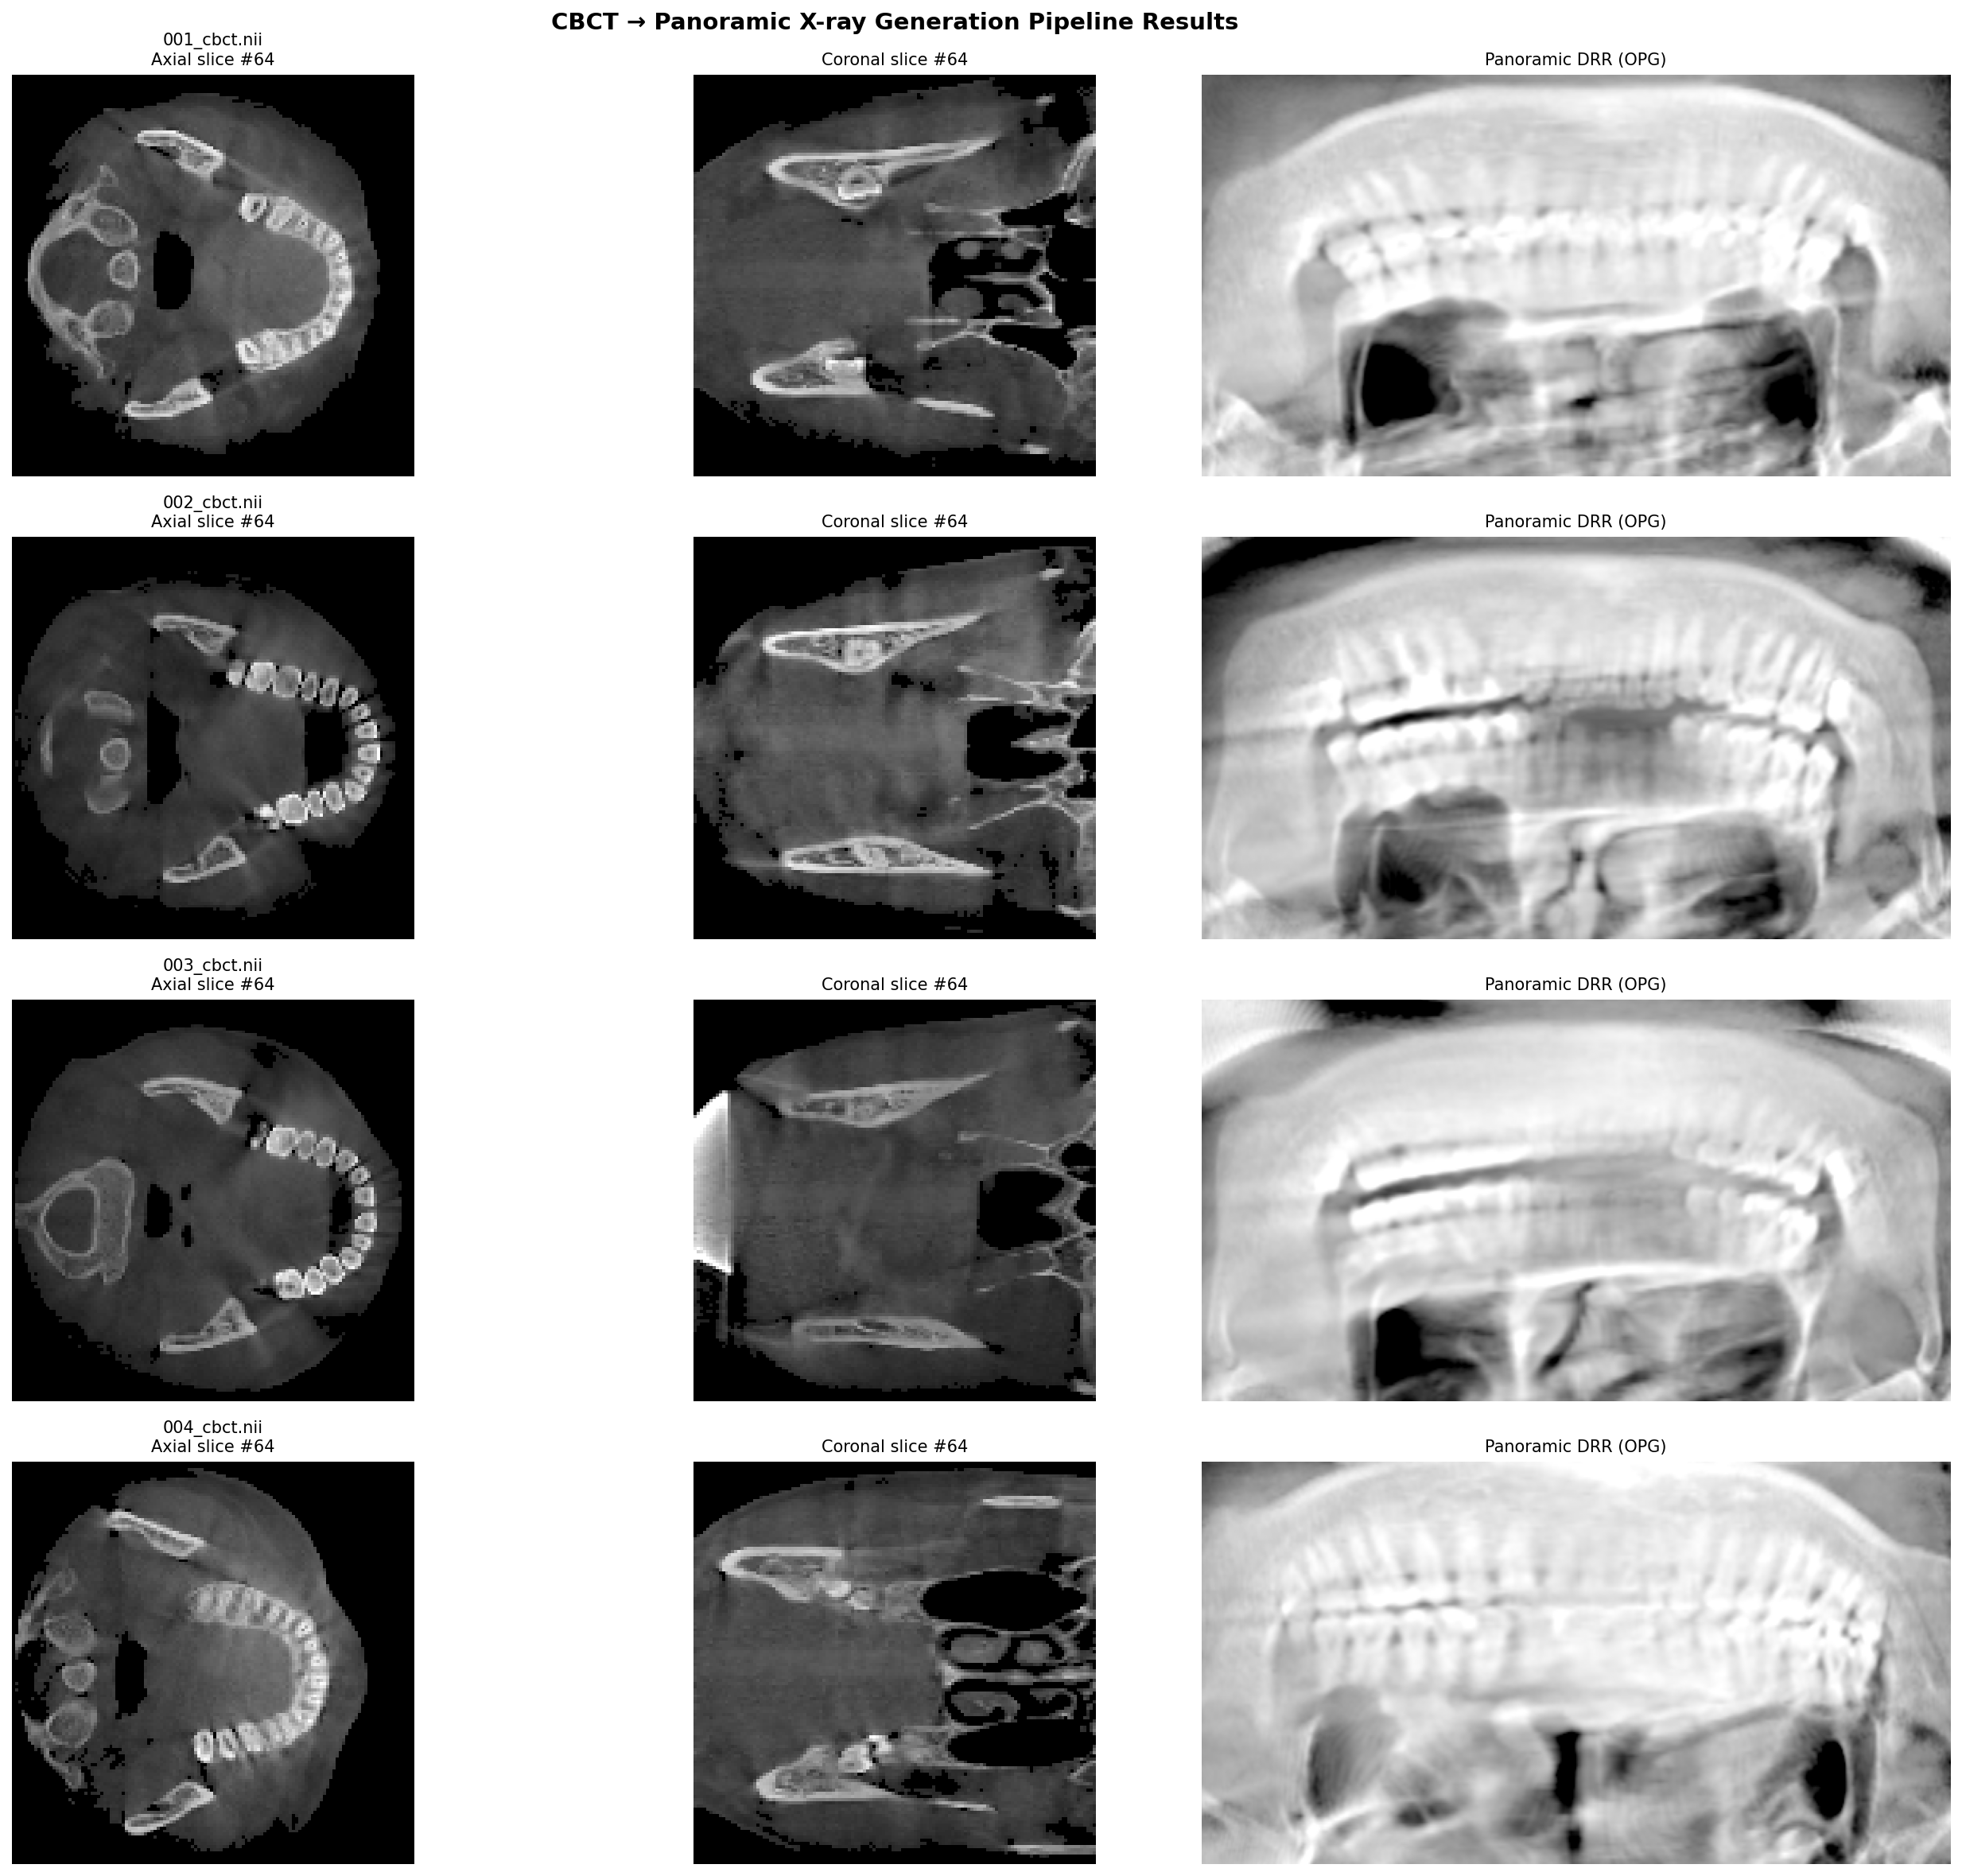
\includegraphics[width=0.96\textwidth]{cbct_to_panoramic_comparison.png}
    \caption{Output showing CBCT slices (axial/coronal) and generated panoramic DRR views}
    \label{fig:results-cbct-to-panoramic}
\end{figure}
\end{frame}

\begin{frame}{Results: Quality Verification Visualization}
\small
\begin{columns}[T,onlytextwidth]
    \begin{column}{0.40\textwidth}
        \textbf{Quality analysis performed}
        \begin{itemize}
            \item Pixel distribution histograms for representative samples.
            \item Center-crop inspection focused on teeth region clarity.
            \item Dynamic range checks (dark/bright fraction).
            \item Contrast consistency analysis across generated panoramics.
        \end{itemize}
    \end{column}
    \begin{column}{0.60\textwidth}
        \begin{figure}
            \centering
            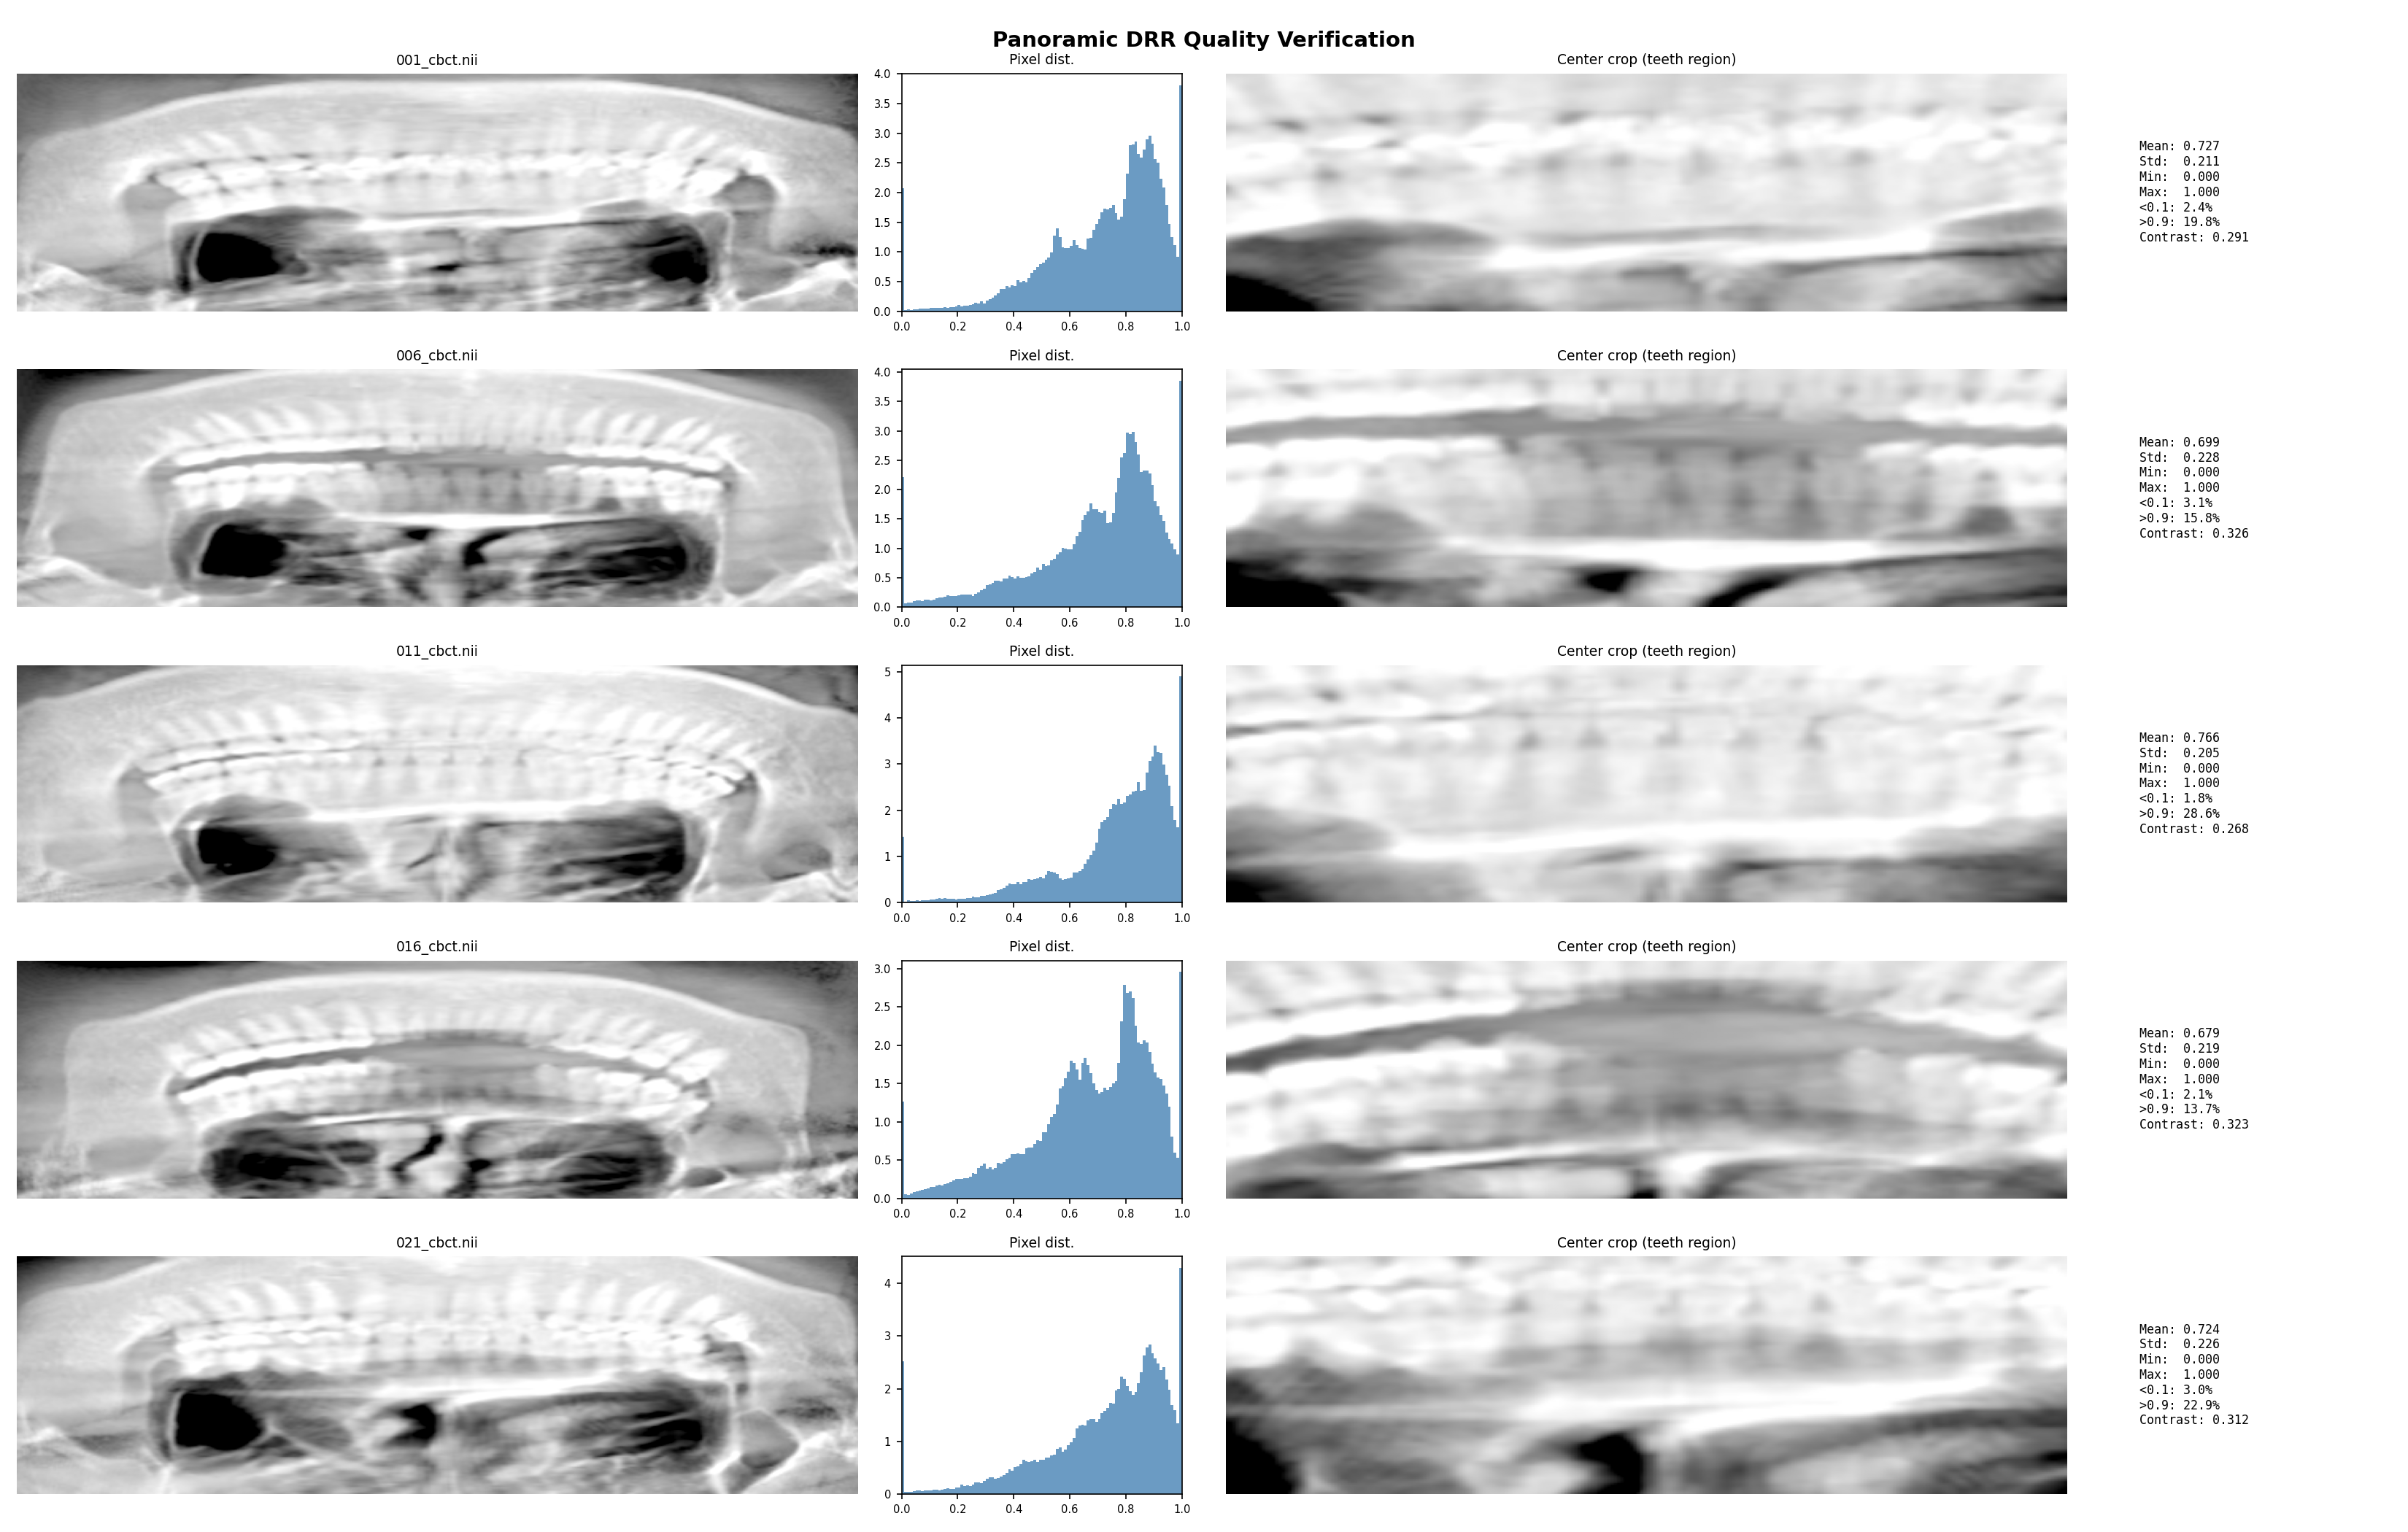
\includegraphics[width=\textwidth]{quality_verification.png}
            \caption{Quality verification panel generated from synthetic panoramic outputs}
            \label{fig:results-quality-verification}
        \end{figure}
    \end{column}
\end{columns}

\end{frame}

\begin{frame}{Future Work}
\begin{itemize}
    \item \textbf{Dynamic Trajectory Estimation:}  
    Develop methods to automatically estimate patient-specific X-ray machine trajectories for improved reconstruction accuracy. \cite{park2024nebla}

    \item \textbf{Multi-Structure Reconstruction:}  
    Extend the current models to reconstruct not only teeth but also jawbones, nerves, and soft tissues.\cite{mildenhall2021nerf}

    \item \textbf{Clinical Integration:}  
    Validate the reconstruction pipeline in real-world clinical workflows such as implant planning and orthodontics.\cite{wang2024neural}

    \item \textbf{Enhanced Generalization:}  
    Improve robustness to artifacts, noise, low-quality X-rays, and diverse patient anatomies.

    \item \textbf{Unified Architecture:}  
    Explore end-to-end architectures that combine explicit approaches (e.g., PX2Tooth) and implicit representations (e.g., Oral-3Dv2).\cite{song2023oral}
\end{itemize}
\end{frame}

\section{References}

\begin{frame}[allowframebreaks]{References}
    \printbibliography
\end{frame}

\end{document}